% ПЛАН
%
%# Глава 2 – Математические основы построения алгоритмов оценки параметров гармоник
%
%Выводы по главе:
%
%1. Математической основой для анализа спектра сигналов является преобразование Фурье. Для дискретных сигналов применяется дискретное преобразование Фурье.
%2. При анализе спектра многотонального сигнала с помощью дискретного преобразования Фурье в большинстве случаев имеются гармоники частота которых не кратна частоте основной гармоники. При оценке их параметров необходимо учитывать изменение спектра сигнала, связанное с ограниченной длиной выборки этого сигнала.
%3. При анализе спектра сигнала с ограниченной выборкой необходимо использовать оконные функции, поскольку в противном случае сигнал будет взвешен прямоугольной оконной функцией с плохой частотной характеристикой.
%4. Применение оконной функции уменьшает количество информации, получаемое из сигнала, и, как следствие, увеличивается дисперсия оценки параметров сигнала, или, другими словами, ухудшается точность оценки параметров сигналов.
%5. Ухудшение точности оценки можно определить исходя из предложенного в главе коэффициента окна. Данный коэффициент показывает, насколько уменьшиться точность оценки амплитуды гармоники для оптимальной несмещенной оценки при применении такого окна, а также может использоваться для оценки снижения точности параметров.
%6. Алгоритмы для нахождения оптимальной несмещенной оценки параметров могут быть построены на основе методов оптимального приема, изучаемых в радиотехники, в частости, с помощью корреляционного анализа.

\chapter{Математические основы построения алгоритмов оценки параметров гармоник} \label{ch:ch2}

Вторая глава посвящена математическим основам построения алгоритмов оценки параметров гармоник.

Спектр сигнала определяется зависимостью сигнала от времени. Временная область и частотная связанны друг с другом с помощью преобразования Фурье. Практически преобразование Фурье определяется с помощью систем цифровой обработки сигналов (ЦОС). Точность гармонических моделей может обеспечить ЦОС, при условии, что математической основой является Дискретное преобразование Фурье (ДПФ, DFT -- Discrete Fourier Transform) или Быстрое преобразование Фурье (БПФ, FFT -- Fast Fourier Transform). 
\cite{Time-frequency_Avramchuk_2009,Optimization_Computational_Altman2008,Building_suboptimal_Altman_2017}
%1. Аврамчук В. С., Гончаров В. И. Чан Вьет Тьяу. Частотно-временной корреляционный анализ цифровых сигналов //Известия Томского политехнического университета. – 2009. – Т. 315. – №. 5. – С. 112-115.
%9. Альтман Е. А. Оптимизация вычислительной схемы быстрого преобразования Фурье //Омский научный вестник. – 2008. – №. 1 (64).
%10. Альтман Е. А. Построение субоптимальных моделей алгоритмов БПФ по основанию 2 //Информационно-телекоммуникационные системы и технологии. – 2017. – С. 409-411.

%ДПФ
\cite{Digital_processing_Sergienko_2011}

Методы цифровой фильтрации сигналов развивались динамично в последние годы. Появились новые математические методы (дискретное преобразование Фурье, быстрое преобразование Фурье, разряженное преобразование Фурье и др.), позволяющие создавать эффективные алгоритмы фильтрации. Фильтрация, в конечном счете, является не конечным этапом обработки сигналов, а предобработкой. Операции могут быть выполнены путем моделирования на персональных компьютерах или с помощью специализированной аппаратуры.
Алгоритмы фильтрации сигналов условно разделяем на два класса:
\begin{itemize}
	\item Алгоритмы фильтрации в пространственной области.
	\item Алгоритмы фильтрации в частотной области.
\end{itemize}



%Статья СРАВНИТЕЛЬНЫЙ АНАЛИЗ ПРИМЕНЕНИЯ АЛГОРИТМОВ ОПРЕДЕЛЕНИЯ ЧАСТОТЫ ПРИ ОЦЕНКЕ ГАРМОНИК В ЭЛЕКТРИЧЕСКИХ СЕТЯХ
Существует большое число алгоритмов определения частоты для оценки гармоник в электрических сетях: ДПФ, интерполированный алгоритм ДПФ (IpDFT -- Interpolated Discrete Fourier Transform), техника заполнения нулями (Zero-crossing), и другие.
\section{Быстрое преобразование Фурье} \label{sec:ch2/sec1}

Применение алгоритмов БПФ началось после публикации работы Джеймса Кули (James Cooley) и Джона Тьюки (John Tukey) в $1965$ году \cite{cooley1965algorithm}. 

В работе Кули и Тьюки была ссылка на публикацию Ирвинга Гуда (Irving Good) \cite{good1958interaction} в $1958$ году, в которой был рассмотрен алгоритм, получивший названияb алгоритм Гуда–Томаса или алгоритм простых чисел. Алгоритм получил известность после публикации Ллевеллина Томаса (Llewellyn Thomas) об использовании этого алгоритма для задач физики \cite{thomas1963using}.

В 1966 году Филип Рудник (Philip Rudnick) опубликовал похожую работу \cite{rudnick1966note}. В ней была ссылка на работу Гордона Даниельсона (Gordon Danielson) и Корнелиуса Ланкоса (Cornelius Lanczos) \cite{danielson1942some} в которой приведены формулы для разложения тригонометрических рядов. 

Научная работа Иоганна Гаусса (Johann Gauss), которая была опубликована после его смерти в сборнике не опубликованных рукописей \cite{gauss1866nachlass}.

Идеи, которые рассмотрены в алгоритме Кули–Тьюки были отрыты
в XIX веке несколько раз. Поэтому сложно предположить кто из авторов первый открыл алгоритм.

Алгоритм БПФ снижает вычислительную сложность ДПФ и применяется, когда количество отсчетов сигнала пропорционально степени $2$ \cite{Quick_conversion_1985}. Исходная последовательность в обобщенном случае может быть другого размера,но данное условие помогает лучше вычислить БПФ. 

БПФ Кули-Тьюки имеет две разновидности: прореживание по времени и частоте \cite{Digital_processing_Goldenberg_1985}. 

В таких алгоритмах $S$-точечная последовательность на первом шаге делится на две $S/2$ последовательности, на следующем шаге каждая из полученных последовательностей делится еще на две равной длины и~т.~д., пока размер не будет равен двум отсчетам. 
Прореживание по времени делит исходную последовательность размером $S$ на две размером $S/2$, состоящие из четных и из нечетных отсчетов. Прореживание по частоте первую последовательность заполняет первыми $S/2$ отсчетами исходной, вторую -- оставшимися $S/2$ отсчетами. На каждом шаге двух вариантов прореживания применяется один и тот же алгоритм. Оба метода имеют схожую структуру, но отличаются весовыми коэффициентами. Поэтому каждый из алгоритмов вычисляет все отсчеты исходной последовательности за одинаковое количество арифметических операций: $(\frac{S}{2})\log2S$ комплексных умножений и $S\log2S$ комплексных сложений.

В последующие годы были разработаны более быстрые алгоритмы вычисления преобразования Фурье. Одними из таких методов при определенных условиях является алгоритм Винограда, теоретико-числовое преобразование.

В качестве главного способа измерения гармоник напряжения 
ГОСТ Р 51317.4.7–2008 \cite{GOSTR51317.4.7-2008} определяет дискретное преобразование Фурье (ДПФ) или быстрое преобразование Фурье (БПФ), которые применяются вместе с дополнительными операциями над данными, например, их сглаживание и взвешивание. Однако это не исключает применение других принципов анализа гармоник \cite{GOSTR51317.4.7-2008}.

Общая структура средств измерений (СИ), рекомендованная в \cite{GOSTR51317.4.7-2008}, реализована на основе БПФ и представлена на рисунке \ref{img:picture7}. 

\begin{figure}[ht]
	\centering
	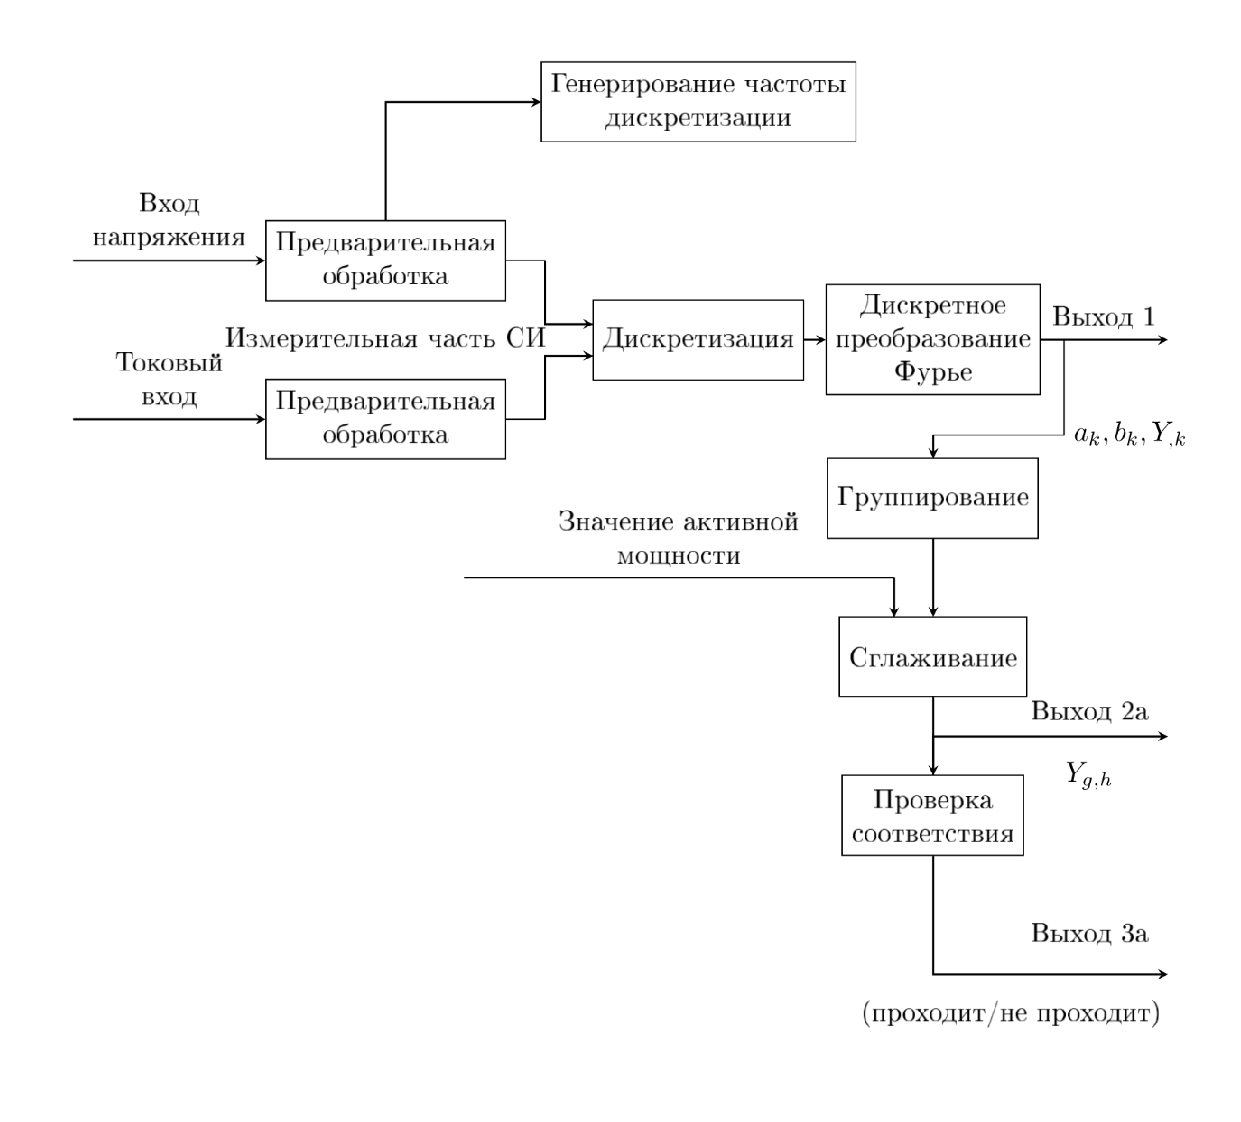
\includegraphics [scale=0.85] {general_SI_structure}
	\caption{Общая структура средств измерений.}
	\label{img:picture7}
\end{figure}

% Математической основой для анализа спектра сигналов является преобразование Фурье. Для дискретных сигналов применяется дискретное преобразование Фурье.

\section{Дискретное преобразование Фурье} \label{sec:ch2/sec2}
Впервые французский математик Ж.Б.Ж. Фурье предположил, что каждую функцию можно разложить в тригонометрический ряд. Эта гипотеза имеет огромное значение в обработке сигналов, то есть периодический сигнал с периодом $T$ может быть представлен суммированием гармонических колебаний с
угловыми частотами $\omega_{n} = n \cdot \omega_{n} $ , где $n$ -- номер гармоники. Гармонику $n = 1$ называют основной гармоникой, а $n > 1$ высшими гармониками. 

Математической основой для анализа спектра сигналов является преобразование Фурье. Для дискретных сигналов применяется дискретное преобразование Фурье.

Чтобы проанализировать алгоритмы определения частоты для оценки гармоник в частотной области часто используют подходы, основанные на дискретном преобразовании Фурье, которые
реализованы с помощью быстрого преобразования Фурье \cite{comparative_analysis_2019}. В формуле \ref{eq:$f(t)$} показано разложение в ряд Фурье периодической функции $f(t)$ с периодом $2\pi$ на интервале $[0,2\pi]$:

\begin{equation}
\label{eq:$f(t)$}
f(t) = \sum_{k=-\infty}^{\infty} {C_{k}\exp^{jkt}},
\end{equation}

где $C_{k}$ -- комплексные коэффициенты Фурье. 

 
\begin{equation}
	\label{eq:$C_{k}$}
	C_{k} = \frac{1}{2\pi} \int\limits_{-\pi}^{\pi} f(t) \exp^{-jkt} \mathrm{d}x,
\end{equation}

где $\bigtriangleup t$ -- интервал дискретизации. 

$N \bigtriangleup t$ -- основной период сигнала. 

 В межгосударственном стандарте \cite{GOST30804.4.7-2013} в качестве способа изменения гармоник напряжения используем ДПФ или БПФ, которые используют дополнительные операции над данными.

Рассмотрим сигнал $x(k)$ с отчетами $N$ для спектра $\dot{X}(n)$. Выражение описывающее ДПФ сигнала имеет следующий вид:
\begin{equation}
	\label{eq:equation1}
	\dot{X}(n)= \displaystyle\sum_{k=0}^{N-1} x(k) \cdot \exp\left( -j \cdot \frac{2 \pi n k}{N}\right).
\end{equation}

Если период равен $T$ для аналогово сигнала кратный расстоянию между отчетами дискретизированного сигнала. То процедура ДПФ обеспечивает точные  параметры для высших гармоник.

Применение дополнительных методов для определения параметров напряжения обусловлено неспособностью ДПФ определить частоту сигнала. На рисунке \ref{img:Maximum_DFT.pdf} показано, что спектр сигнала не совпадает с максимумом спектра напряжения \cite{Definition_parameters_Altman_2012, Digital_processing_Sergienko_2011}. 
\begin{figure}[p]
	\centering
	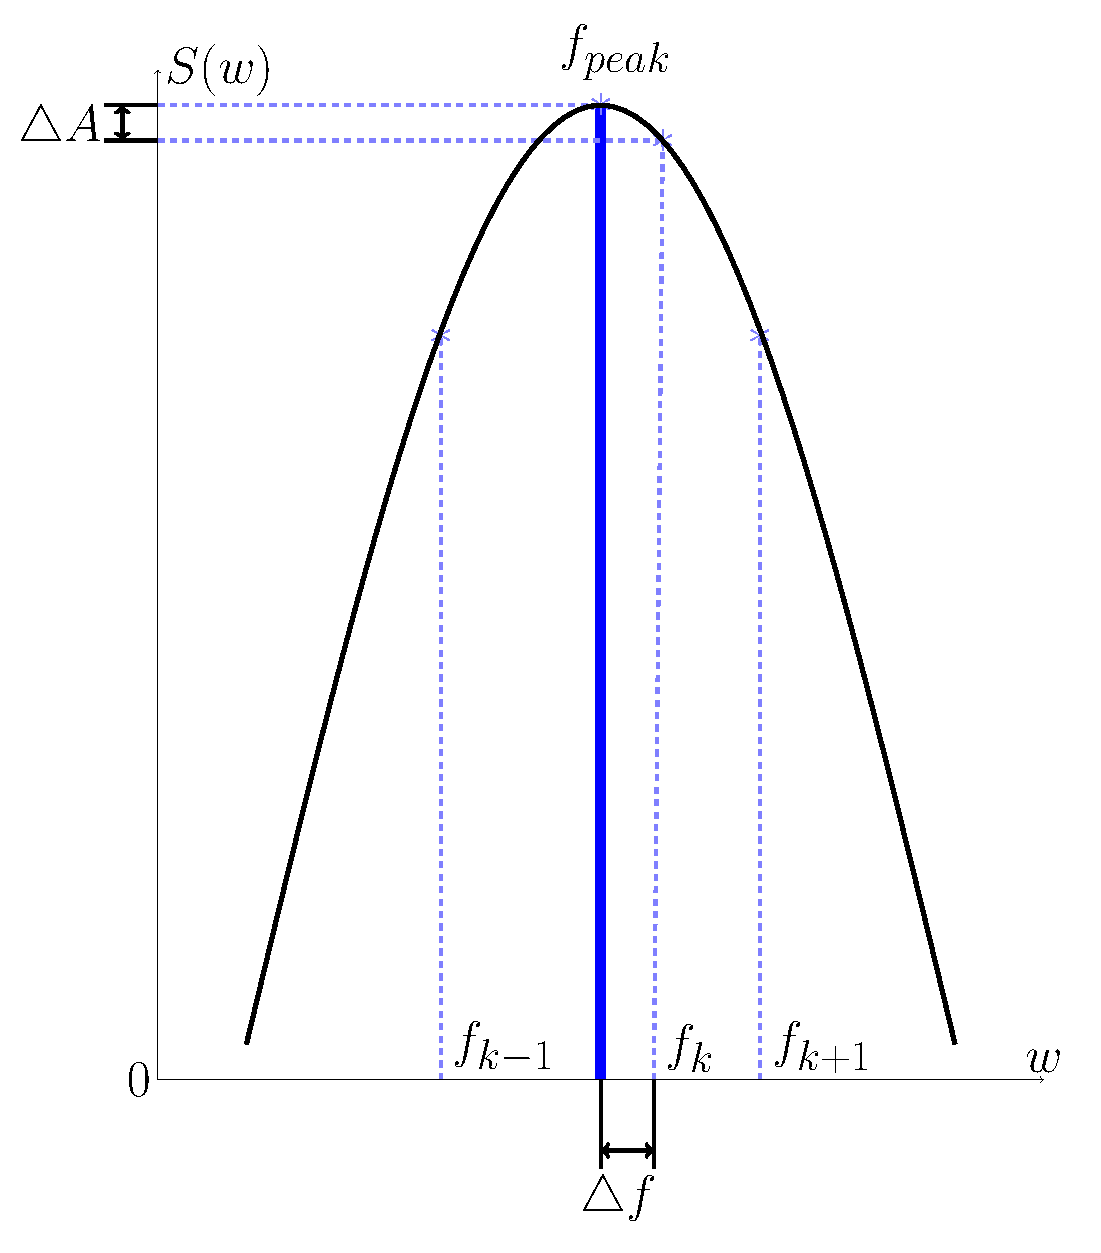
\includegraphics [scale=0.5] {Maximum_DFT.pdf}
	\caption{Несовпадение максимума спектра напряжения и максимума ДПФ.}
	\label{img:Maximum_DFT.pdf}
\end{figure}
На рисунке \ref{img:Maximum_DFT.pdf} обозначим максимум ДПФ -- $k$, $k-1$, $k+1$ -- вершины. $k_{peak}$ -- порядковый номер гармоники спектра напряжения. Диапазон между максимумо ДПФ и порядковым номером максимальной гармоники обозначим $\delta$

ДПФ широко используемая вычислительная задача. Приложения его включают обработку сигналов, сжатие аудио/изображений/видео. 

В настоящее время быстрым алгоритмом является БПф, который вычисляет ДПФ $n$-мерного сигнала за время $O(n \log n)$. Существование алгоритмов ДПФ быстрее, чем БПФ.

\section{Нижняя граница Крамера-Рао} \label{sec:ch2/sec3} %АНТИПЛАГИАТ=
% Альтман Е. А., Васеева Т. В., Александров А. В. ГРАНИЦА КРАМЕРА-РАО ДЛЯ АМПЛИТУДЫ ГАРМОНИКИ ПРИ ИСПОЛЬЗОВАНИИ ОКОННЫХ ФУНКЦИЙ //Динамика систем, механизмов и машин. – 2020. – Т. 8. – №. 2. – С. 145-152.
% ВВЕДЕНИЕ 
Для определения точности полученных результатов алгоритмы можно проверить с помощью неравенства Крамера-Рао. В зарубежной литературе чаще встречается термин Cramer-Rao lower bound (CRLB), что обозначает <<нижняя граница Крамера-Рао>>. В неравенстве Крамера-Рао сигнал имеет наибольшую величину дисперсии при некоторых условиях. Если неравенство Крамера-Рао преобразуется в равенство, то оценка параметров считается наилучшей. Отсюда следует, что дисперсия данной оценки самая маленькая из возможных. 

Несмещенная оценка, которая достигается нижней границей Крамера-Рао, называется эффективной. Такое решение обеспечивает наименьшую среднеквадратичную ошибку среди несмещенных методов и называется minimum variance unbiased (MVU)~--~<<оценкой с минимальной несмещенной дисперсией>> \cite{altman2020boundary}.

Информация Фишера играет важную роль в статическом моделировании для построения гипотез с использованием оценок максимального правдоподобия. Функция правдоподобия называется maximum likelihood estimation (MLE), то есть <<оценкой максимального правдоподобия>>. Если можно найти производную из функции правдоподобия, то решение первого порядка производной функции возможно с помощью метода наименьших квадратов. Чаще используют методы определения локальных максимумов и минимумов с помощью численных методов \cite{press1992art}.

% 14. Press, W. H.; Flannery, B. P.; Teukolsky, S. A.; Vetterling, W. T. (1992). "Least Squares as a Maximum Likelihood Estimator". Numerical Recipes in FORTRAN: The Art of Scientific Computing (2nd ed.). Cambridge: Cambridge University Press. pp. 651–655. ISBN 0-521-43064-X.

Формирование уравнений для получения оценки и вычисления ее дисперсии можно решать формирование по методу максимального правдоподобия. Известно \cite{kay1993fundamentals}, что максимально правдоподобные оценки асимптотически состоятельны и эффективны, то есть их дисперсия совпадает с нижней границей Крамера-Рао. В источнике \cite{kay2013fundamentals} представлена классификация существующих алгоритмов оценки. Также следует отметить, что решения алгоритмов зависят от того, считается ли сигнал детерминированным или результатом случайного процесса. Предложенная формула в статье позволяет выбирать оконную функцию для решения задач спектрального анализа и дает оценку дисперсии амплитуды при выборе метода.

% 12. Kay S. M. Fundamentals of statistical signal processing. – Prentice Hall PTR, 1993.
% 13. Kay S. M. Fundamentals of statistical signal processing: Practical algorithm development. – Pearson Education, 2013. – Т. 3.
%МАТЕМАТИЧЕСКАЯ МОДЕЛЬ ДЛЯ ОЦЕНКИ ТОЧНОСТИ НАХОЖДЕНИЯ АМПЛИТУДЫ ГАРМОНИКИ
В общем случае граница Крамера-Рао определяется следующим образом \cite{kay1993fundamentals, kay2013fundamentals}:
% 12. Kay S. M. Fundamentals of statistical signal processing. – Prentice Hall PTR, 1993.
%13. Kay S. M. Fundamentals of statistical signal processing: Practical algorithm development. – Pearson Education, 2013. – Т. 3.

\begin{equation}
	\label{eq:equation1}
	var(\theta)\geq\frac{1}{-E\left[\frac{(\delta^2 ln p(x;\theta)}{\delta\theta^2}\right]}
\end{equation}

где $\theta$ -- оцениваемый параметр; 

var($\theta$) -- дисперсия (variance) несмещенной оценки параметра;

$E$ -- среднее значение;

$p(x;\theta)$ -- функция правдоподобия.

Формулу ~(\ref{eq:equation1}) при выполнении условия регулярности функции правдоподобия можно разделить на части и записать в следующем виде:

\begin{equation}
	\label{eq:equation2}
	var(\theta)\geq\frac{1}{I(\left.\theta)\right]}
\end{equation}

где $I(\theta)=-E\left[\frac{\delta^2 ln p(x;\theta)}{\delta\theta^2}\right]$ -- количество информации по Фишеру, получаемой в результате наблюдения.

По формуле ~(\ref{eq:equation2}) хорошо просматривается физический смысл границы Крамера-Рао: дисперсия оценки параметра обратно пропорциональна количеству информации, полученному в результате наблюдения.

При наблюдении за дискретным сигналом, на который накладывается аддитивный белый гауссовский шум, формула (\ref{eq:equation1}) может быть записана в виде: 

\begin{equation}
	\label{eq:equation3}
	var(\theta)\geq\frac{\sigma^2}{\sum_{n=0}^{N-1}\left(\frac{\delta x(n;\theta)}{\delta\theta}\right)^2}
\end{equation}

где $\sigma $ -- среднее квадратичное отклонение шума;

N -- число отсчетов в дискретном сигнале;

$x(n;\theta)$ -- наблюдаемый сигнал.

В нашем случае наблюдаемый сигнал описывается следующей формулой:
\begin{equation}
	\label{eq:equation4}
	x_n=A\cos(2*\pi*f*n+\phi)+wgn_n, n\in0,…,n-1
\end{equation}

где $A$ -- амплитуда сигнала;

$f$ -- частота;

$\phi$ -- фаза;

$wgn$ -- белый гауссовский шум.

Этот сигнал содержит три неизвестных параметра (амплитуду, частоту и фазу). Строго говоря, в данном случае нужно применять векторный вариант формулы для границы Крамера-Рао, однако, как показано в \cite{kay1993fundamentals}, при условии, что частота сигнала не находится вблизи от частот равных нулю или половине частоты дискретизации, влияние неопределенности частоты и фазы сигнала на неопределенность амплитуды пренебрежимо мало.

Пренебрегая неопределенностью частоты и фазы получим следующую формулу для дисперсии оценки амплитуды гармоники в аддитивном белом гауссовском шуме: 

\begin{equation}
	\label{eq:equation5}
	I(A)=\sum_{n=0}^{N-1}\left( \frac{\delta x}{\delta A} \right)^2 =\frac{1}{\sigma^2} \sum_{n=0}^{N-1}\cos^2 (2*\pi*f*n+\phi)\approx \frac{N}{2\delta ^2 }
\end{equation}

После применения оконной функции сигнал будет записан в виде: 

\begin{equation}
	\label{eq:equation6}
	x_n^{'}= w_n*A\cos(2*\pi*f*n+\phi)+w_n*wgn_n,..n\in 0,…,n-1
\end{equation}
где $w$ -- оконная функция.

Рассмотрим слагаемые в формуле ~(\ref{eq:equation6}) по отдельности. Слагаемое $w_n*wgn_n$ будет представлять собой нормально распределенную случайную величину с нулевым математическим ожиданием. Определим дисперсию этой случайной величины.

Во всех $n\in 0,…,n-1$ отклонение от нуля будет нормально распределено со средним отклонением равным $w_n*\sigma$. Среднее квадратичное отклонение в каждой точке будет равно $w_n^2*\sigma^2$. Усредняя по всем n получаем, что дисперсия случайной величины $w_n*wgn_n$ будет: 

\begin{equation}
	\label{eq:equation7}
	\sigma^{'2}=\frac{\sum_{n=0}^{N-1} w_n^2}{N}*\sigma^2
\end{equation}

Теперь, для нахождения дисперсии результата оценки амплитуды, мы можем воспользоваться формулой (\ref{eq:equation1}) и подставить в нее новую дисперсию шума $\sigma^{'^2}$.

Рассмотрим знаменатель правой части формулы. Для упрощения выкладок воспользуемся трансформацией параметра при определении границы Крамера-Рао \cite{kay1993fundamentals,kay2013fundamentals}. Если величина $\alpha$, которую нужно оценить, связана с величиной $\theta$, для которой известна граница Крамера-Рао, соотношением $\alpha=g(\theta)$, то границу Крамера-Рао для величины $\alpha$ можно найти по формуле: 

\begin{equation}
	\label{eq:equation8}
	var(\theta)\geq \frac{\left(\frac{\delta^2 g}{\delta\theta}\right)}{-E\left[\frac{\delta^2 ln p(x;\theta)}{\delta \theta^2}\right]^{'}}
\end{equation}

Умножение сигнала на оконную функцию приводит к сворачиванию каждой гармоники сигнала со спектром оконной функции. В случае единственной гармоники ее амплитуда умножается на нулевую гармонику спектра оконной функции. Нулевая гармоника сигнала это постоянная составляющая, ее значение для оконной функции можно найти по формуле: 

\begin{equation}
	\label{eq:equation9}
	w_0= \frac{\sum_{n=0}^{N-1} w_n}{N}.	  
\end{equation}

Получаем, что: 
\begin{equation}
	\label{eq:equation10}
	A^{'}=\frac{A}{w_0} ,		  
\end{equation}

где A -- амплитуда гармоники, полученная в результате оценки умноженного на оконную функцию сигнала; 

$A^{'}$ -- амплитуда гармоники исходного сигнала.

В нашем случае величина $\theta$ с известной границей Крамера-Рао это A, величина $\alpha$ с неизвестной границей это  $A^{'}$ , $g(\theta)=\frac{\theta}{w_0}, \left(\frac{\delta^2 g}{\delta \theta}\right)^2=\frac{1}{w_0^2}$.

Собирая все полученные соотношения вместе, получим формулу для дисперсии оценки амплитуды гармоники при использовании оконной функции: 
\begin{equation}
	\label{eq:equation11}
	var(A)\geq \frac{2\sigma^2}{N} \frac{\sum_{n=0}^{N-1}w_n^2}{\left(\sum_{n=0}^{N-1} w_n \right)^2} 			  
\end{equation}

%5. Ухудшение точности оценки можно определить исходя из предложенного в главе коэффициента окна. Данный коэффициент показывает, насколько уменьшиться точность оценки амплитуды гармоники для оптимальной несмещенной оценки при применении такого окна, а также может использоваться для оценки снижения точности параметров.

С практической точки зрения имеет смысл выделить из этой формулы вторую часть. Введем обозначение коэффициент окна: 
\begin{equation}
	\label{eq:equation12}
	F_{win}=\frac{\sum_{n=0}^{N-1}w_n^2}{\left(\sum_{n=0}^{N-1} w_n\right)^2}
\end{equation}

Данный коэффициент показывает, во сколько ухудшится оценка амплитуды гармоники при использовании окна $w$.
% РЕЗУЛЬТАТЫ ЭКСПЕРИМЕНТОВ
Для проверки правильности рассмотренных выкладок мы промоделировали измерение амплитуды гармоник в однотональном сигнале. Экспериментально были проверены формулы (\ref{eq:equation7}) (оценка дисперсии белого шума после наложения на него окна) и (\ref{eq:equation11}) (оценка дисперсии амплитуды гармоники). Для формулы (\ref{eq:equation11}) были построены два графика -- дисперсия в зависимости от окна и от уровня шума.

Зависимость дисперсии сигнала с шумом от дисперсии сигнала с наложенным на него окном (окно Кайзера с параметром $kaiser\_beta$) приведена на рисунке \ref{img:noise_win_var}.

Основная часть программы для оценки дисперсии белого шума после наложения на него окна представлена в приложении \ref{app:Г}. Здесь $np$ это импортированная библиотека numpy, $variances$ -- массив исходных значений дисперсий белого шума.
\begin{figure}[ht]
	\centerfloat{
		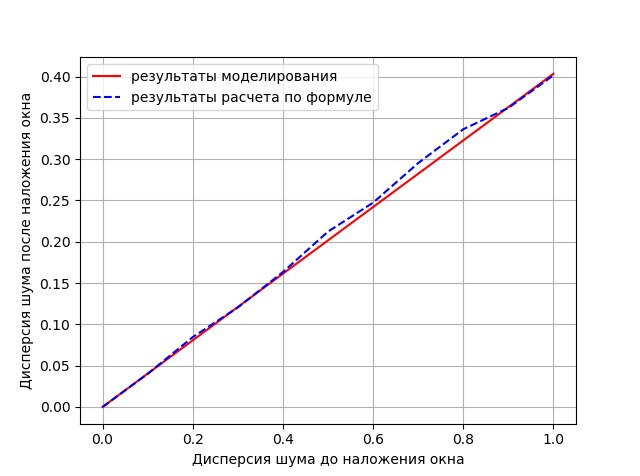
\includegraphics[scale=0.9]{noise_win_var.png}
	}
	\caption{Зависимость дисперсии шума после наложения окна от параметра окна.}\label{img:noise_win_var}
\end{figure}
Использовались параметры $kaiser\_beta=5$ и $n\_point = 1000$ и $n\_test = 100$.
Сплошной линией отображены результаты моделирования, штриховой -- результаты расчета по формуле (\ref{eq:equation7}).

Результаты моделирования при других параметрах аналогичны. Моделирование оценки амплитуды при использовании разных окон проводилось с использованием окна Кайзера с различными параметрами бета. При различных бета данное окно обладает свойствами, сопоставимыми со всеми другими окнами, поэтому полученные результаты справедливы для всех окон (приложение \ref{app:Д}). 
Результаты моделирования приведены на рисунке \ref{img:estimate_amp_sin_kaiser_beta}. 
\begin{figure}[ht]
	\centerfloat{
		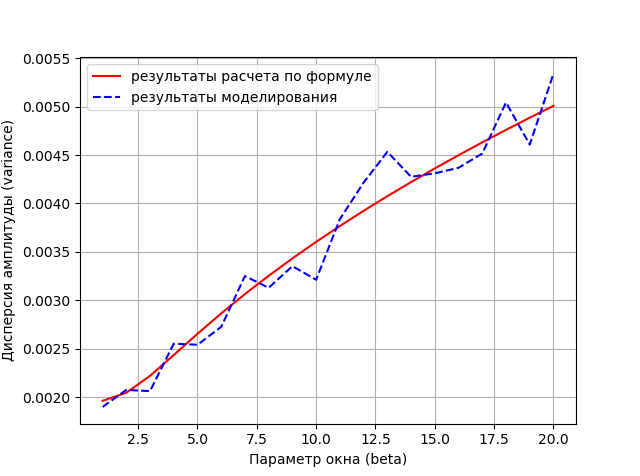
\includegraphics[scale=0.9]{estimate_amp_sin_kaiser_beta.png}
	}
	\caption{Зависимость дисперсии оценки амплитуды от параметра окна.}\label{img:estimate_amp_sin_kaiser_beta}
\end{figure}

Сплошной линией показаны расчеты по формуле (\ref{eq:equation11}), штриховой -- результаты моделирования. При увеличении числа тестов рисунки становятся все более одинаковыми. Результаты моделирования приведены на рисунке \ref{img:estimate_amp_sin_kaiser_noise}. Программа для моделирования оценки амплитуды при различных уровнях шума приведена в приложении \ref{app:Е}.
\begin{figure}[ht]
	\centerfloat{
		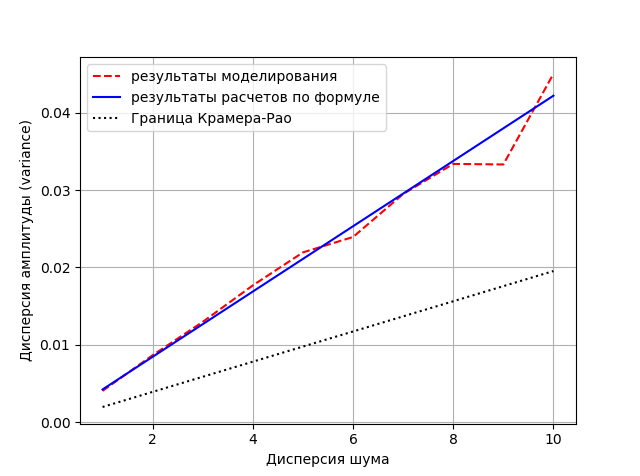
\includegraphics[scale=0.9]{estimate_amp_sin_kaiser_noise.png}
	}
	\caption{Зависимость дисперсии оценки амплитуды от дисперсии шума.}\label{img:estimate_amp_sin_kaiser_noise}
\end{figure}

Штриховой линией приведены результаты расчетов по формуле (\ref{eq:equation11}), сплошной -- результаты моделирования, линией из точек -- граница Крамера-Рао.

%ОБСУЖДЕНИЕ РЕЗУЛЬТАТОВ
Оценку точности результатов для данных, которые сами по себе являются оценкой точности, выполнить на прямую довольно затруднительно. Для проверки точности и достоверности результатов все эксперименты повторялись с различным числом опытов (величина $n\_test$ в программах). Во всех трех экспериментах с увеличением числа опытов экспериментальные кривые сглаживались и становились визуально не отличимые от расчетных данных.

Эксперименты были проведены при различных входных параметрах (число точек, амплитуда, частота и фаза сигналов, дисперсия шума или коэффициент окна). Ни в одном случае не было зафиксировано отклонение результатов эксперимента от результатов, полученных по предложенной формуле.

Таким образом, результаты моделирования алгоритма оценки амплитуды гармоники в условиях шума при наложении оконной функции подтверждают полученные соотношения для оценки дисперсии оценки амплитуды.

%ВЫВОДЫ И ЗАКЛЮЧЕНИЕ
В работе получена формула для оценки дисперсии амплитуды при ее оценке с помощью оптимального несмещенного метода с использованием оконной функции.

Эта формула дает оценку дисперсии при использовании метода, вносящего оптимальную несмещенную оценку. К таким методам относится корреляционный анализ на основе БПФ, который чаще всего и используется при решении задач спектрального анализа.

Предложенная формула может использоваться при выборе оконной функции для решения задач спектрального анализа. Точность получаемой оценки амплитуды – это не единственный критерий при таком выборе, но этот критерий часто является наиболее значимым.

Она также может использоваться на стадии оценки точности выработанного алгоритма анализа спектра сигнала, для оценки уровня шума и в других смежных задачах.

Используемый в работе подход для нахождения дисперсии результата алгоритма обработки сигналов может быть применен и для других задач обработки сигналов, в которых применяются оконные функции или другие предварительные преобразования сигнала.

\section{Граница Крамера-Рао амплитуды однотонального сигнала для методов ее оценки с использованием оконных функций} \label{sec:ch2/sec4} %АНТИПЛАГИАТ=90,62%
% Васеева Т. В., Альтман Е. А. ГРАНИЦА КРАМЕРА-РАО АМПЛИТУДЫ ОДНОТОНАЛЬНОГО СИГНАЛА ДЛЯ МЕТОДОВ ЕЕ ОЦЕНКИ С ИСПОЛЬЗОВАНИЕМ ОКОННЫХ ФУНКЦИЙ //Инновационные проекты и технологии в образовании, промышленности и на транспорте. – 2021. – С.

Граница Крамера-Рао позволяет найти минимальную дисперсию оценки параметра сигнала. Для гармонических сигналов известны различные формулы, которые оценивают параметры: дисперсии амплитуды, частоты и фазы гармоник. Известные алгоритмы оценки показывают результаты выше границы Крамера-Рао. В проведенных исследованиях \cite{altman2020boundary} вывелась формула для оценки минимальной дисперсии амплитуды гармоник для методов, использующих оконные функции. В данной статье более подробно рассмотрели влияние различных окон на сигнал. Полученные результаты позволят решать задачи выбора оконной функции для спектрального анализа.

Модель напряжения $u_{t}$ рассматривается как сумма элементарных синусоидальных сигналов разных частот (1), которые кратны основной частоте, с наложенным аддитивным белым гауссовым шумом 
%η(t):

\begin{equation}
	\label{eq:equation13}
	u(t)=\sum_{v=0}^{v=N}A_{v}\cos \left( \frac{2 \pi}{T_{s}}vt + \varphi_{v} \right) + \eta(t)
\end{equation}

где $A_{v}$ -- амплитуда $v$-й гармоники;

$\varphi_{v}$ -- фаза $v$-й гармоники;

$T_{s}$ -- период.

Процесс наложения окна представляет собой умножение напряжения $u(t)$ на весовую функцию $w(t)$ (рисунок \ref{img:blending_process _and_Hamming_window}). Основная цель наложения окна -- получить ограниченную во времени функцию, при минимальных спектральных искажения. В зарубежной литературе так же называют спектральная утечка.
\begin{figure}[ht]
	\centerfloat{
		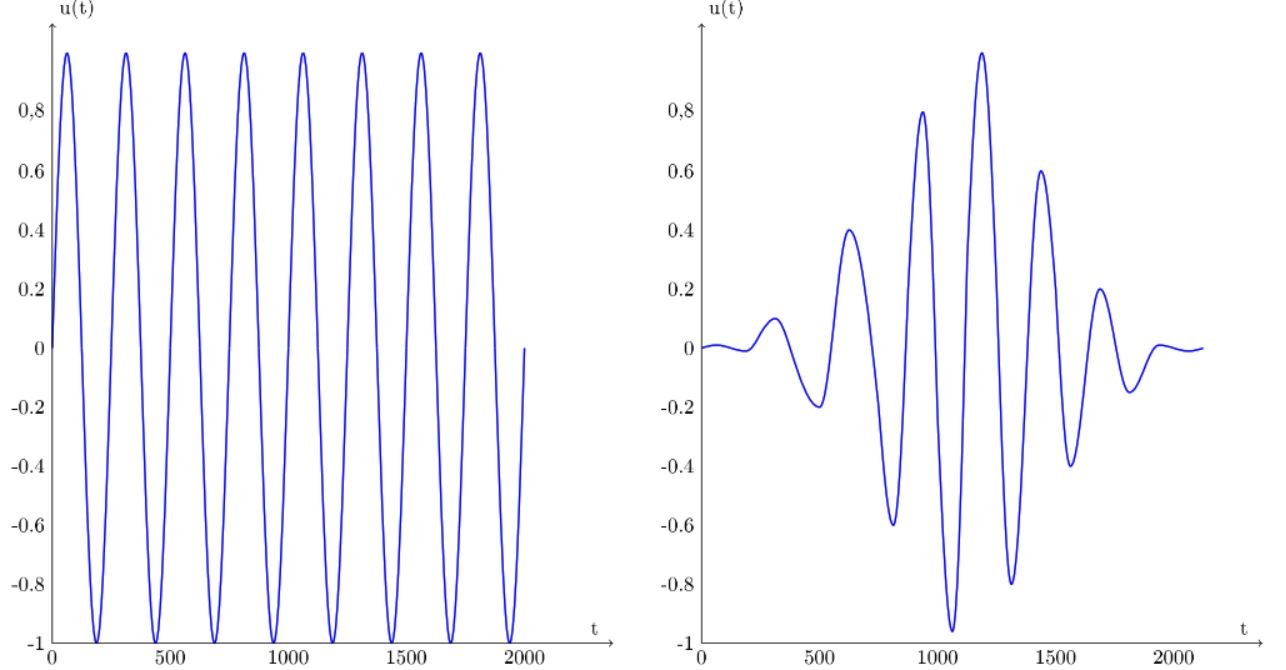
\includegraphics[scale=0.6]{blending_process_and_Hamming_window.JPG}
	}
	\caption{а – Напряжение до наложения на него окна Хемминга (слева), б – Напряжение после наложение на него окна.}\label{img:blending_process _and_Hamming_window}
\end{figure}

Рассмотрим оконные функции: Кайзера, Барлетта, Ханна, Хэмминга, Блэкмана (рисунок \ref{img:Windows}, приложение \ref{app:А}) \cite{comparative_study2020,Increase_Accuracy_Yelizarov2014}. 
%2. Васеева Т. В., Альтман Е. А., Александров А. В. Сравнительное исследование гармонических и интергармонических методов оценки сигналов //Инновационные проекты и технологии в образовании, промышленности и на транспорте. – 2020. – С. 51-57.
%3. Елизаров Д. А. Повышение точности оценки показателей несинусоидальности напряжения в электроэнергетических системах //Омск: дис.… канд. техн. наук. – 2014.

\begin{figure}[ht]
	\centerfloat{
		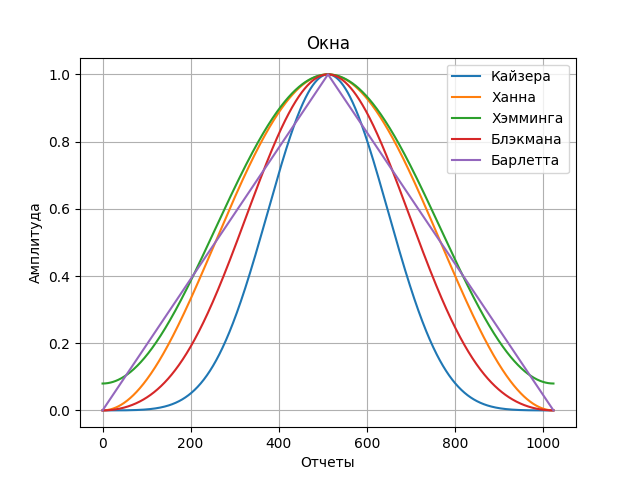
\includegraphics[scale=0.9]{Windows.png}
	}
	\caption{Окна: Кайзера ($\beta=15$), Ханна, Хэмминга, Блэкмана, Барлетта .}\label{img:Windows}
\end{figure}
Умножение сигнала на оконную функцию приводит сворачиванию каждой гармоники со спектром оконной функции. Дисперсии оценки увеличивается из-за наложения на исходный сигнал оконных функций. 

Точность полученных результатов можно проверить с помощью неравенства Крамера-Рао (CRLB -- Cramer-Rao lower bound). В неравенстве Крамера-Рао сигнал имеет наибольшую величину дисперсии при некоторых условиях. Если неравенство Крамера-Рао преобразуется в равенство, то оценка параметров считается наилучшей. Отсюда следует, что дисперсия данной оценки самая маленькая из возможных.

В статье \cite{altman2020boundary} мы промоделировали измерение амплитуды гармоник в однотональном сигнале. Была проверена формула \ref{eq:equation7} оценки дисперсии белого шума после наложения на него окна:
% 1. Альтман Е. А., Васеева Т. В., Александров А. В. Граница Крамера-Рао для амплитуды гармоники при использовании оконных функций //Динамика систем, механизмов и машин. – 2020. – Т. 8. – №. 2. – С. 145-152.

Зависимость дисперсии сигнала с шумом от дисперсии сигнала с наложенным на него окном приведены на рисунке 3. Использовались параметры: $n\_point = 1000$ и $n\_test = 100$. Сплошной линией отображены результаты моделирования, штриховой -- результаты расчета по формуле \ref{eq:equation7}. Результаты моделирования при других параметрах аналогичны.


\begin{figure}[ht]
	\centerfloat{
		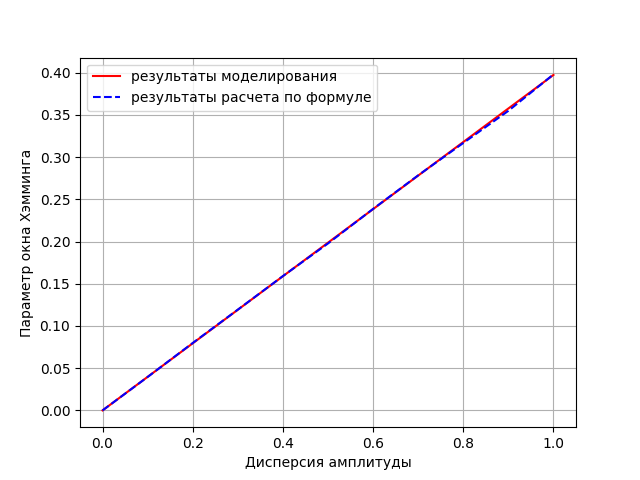
\includegraphics[scale=0.9]{noise_win_var_hamming.png}
	}
	\caption{Зависимость дисперсии шума после наложения окна от параметра окна Хэмминга.}\label{img:noise_win_var_hamming}
\end{figure}

Экспериментально проверили формулу \ref{eq:equation11} оценки дисперсии амплитуды гармоники в статье \cite{altman2020boundary}.
% 1. Альтман Е. А., Васеева Т. В., Александров А. В. Граница Крамера-Рао для амплитуды гармоники при использовании оконных функций //Динамика систем, механизмов и машин. – 2020. – Т. 8. – №. 2. – С. 145-152.

Результаты моделирования приведены на графиках. 
\begin{figure}[ht]
	\centerfloat{
		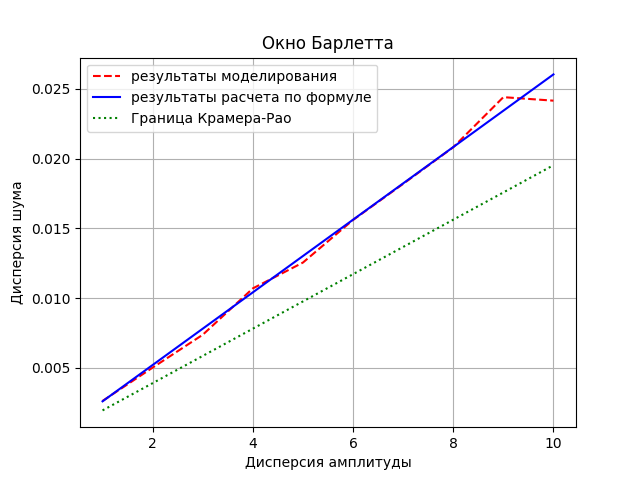
\includegraphics[scale=0.9]{estimate_amp_sin_barlett_noise.png}
	}
	\caption{Зависимость дисперсии оценки амплитуды от дисперсии шума с окном Барлетта.}\label{img:windows_barlett}
\end{figure}

\begin{figure}[ht]
	\centerfloat{
		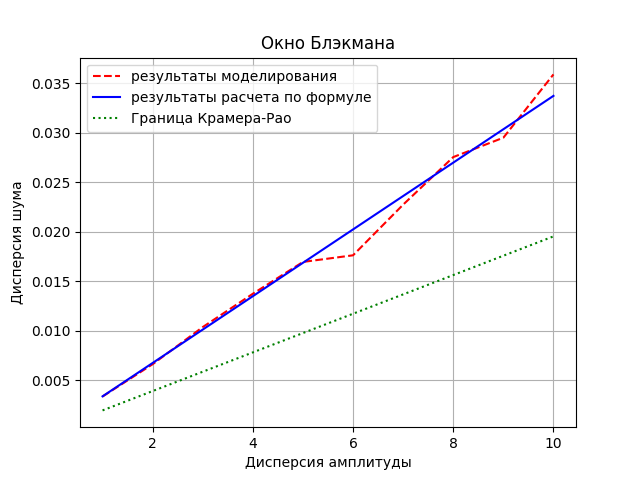
\includegraphics[scale=0.9]{estimate_amp_sin_blackman_noise.png}
	}
	\caption{Зависимость дисперсии оценки амплитуды от дисперсии шума с окном Блэкмана.}\label{img:windows_blackman}
\end{figure}

\begin{figure}[ht]
	\centerfloat{
		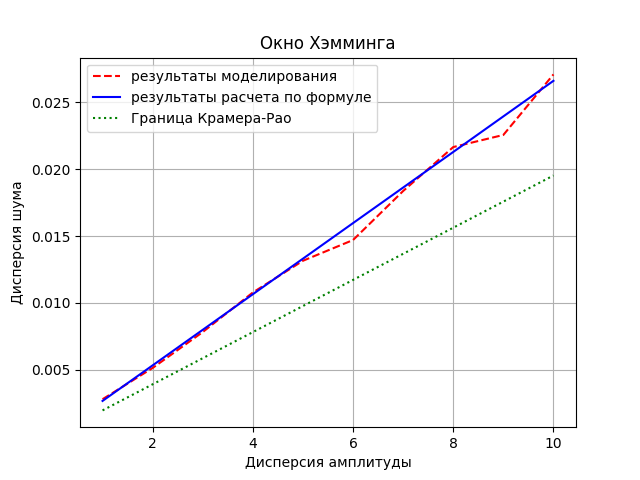
\includegraphics[scale=0.9]{estimate_amp_sin_hamming_noise.png}
	}
	\caption{Зависимость дисперсии оценки амплитуды от дисперсии шума с окном Хэмминга.}\label{img:windows__hamming}
\end{figure}

\begin{figure}[ht]
	\centerfloat{
		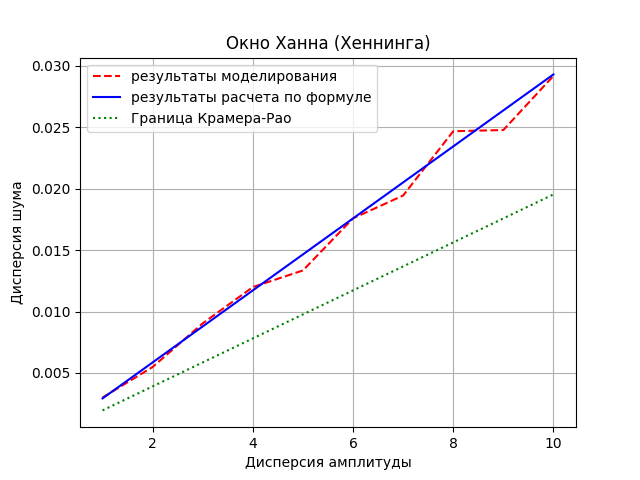
\includegraphics[scale=0.9]{estimate_amp_sin_hanning_noise.png}
	}
	\caption{Зависимость дисперсии оценки амплитуды от дисперсии шума с окном Ханна.}\label{img:windows_hanning}
\end{figure}

\begin{figure}[ht]
	\centerfloat{
		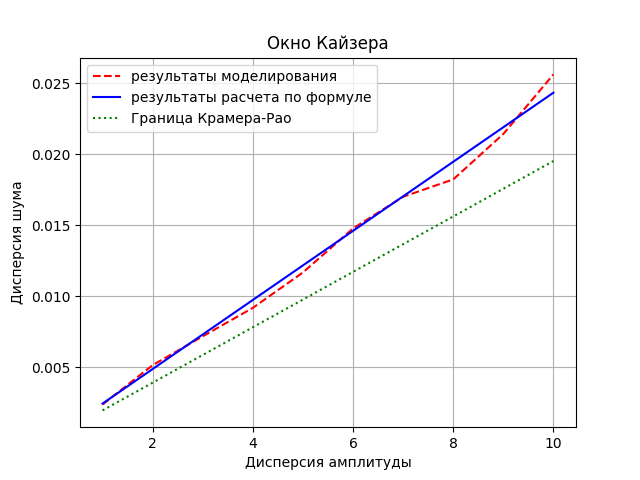
\includegraphics[scale=0.9]{estimate_amp_sin_kaiser(beta=4)_noise.png}
	}
	\caption{Зависимость дисперсии оценки амплитуды от дисперсии шума с окном Кайзера ($\beta=4$).}\label{img:windows__kaiser4}
\end{figure}

\begin{figure}[ht]
	\centerfloat{
		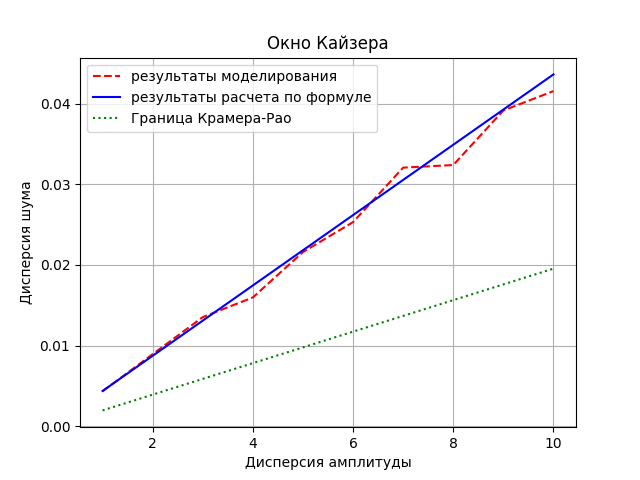
\includegraphics[scale=0.9]{estimate_amp_sin_kaiser(beta=15)_noise.png}
	}
	\caption{Зависимость дисперсии оценки амплитуды от дисперсии шума с окном Кайзера ($\beta=15$).}\label{img:windows__kaiser15}
\end{figure}

%\begin{figure}[ht]
%	\begin{minipage}[b][][b]{0.65\linewidth}\centering
%		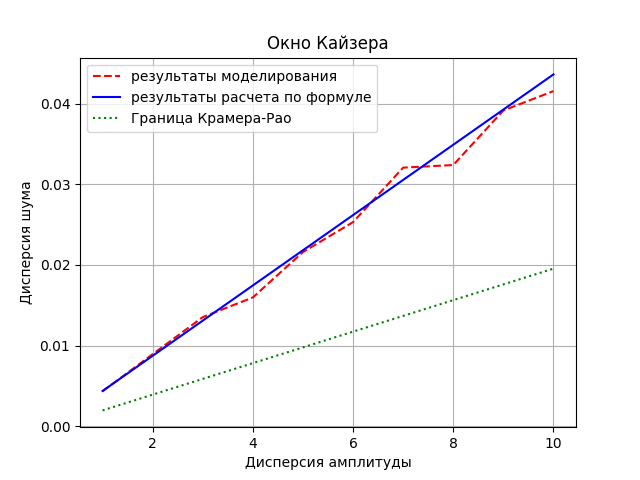
\includegraphics[width=0.5\linewidth]{estimate_amp_sin_kaiser(beta=15)_noise.png} \\ а)
%	\end{minipage}
%	\hfill
%	\begin{minipage}[b][][b]{0.65\linewidth}\centering
%		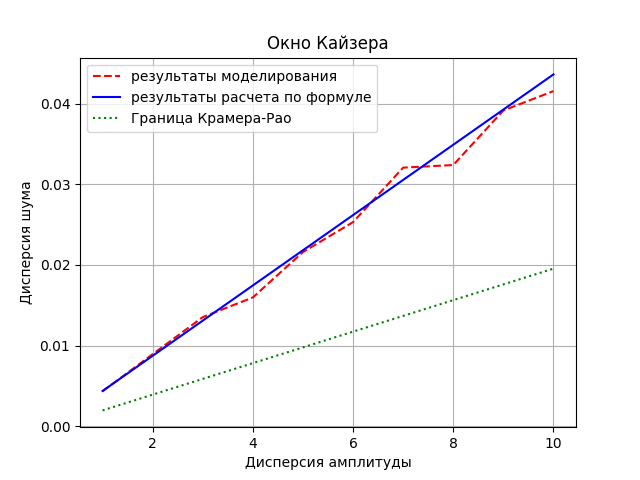
\includegraphics[width=0.5\linewidth]{estimate_amp_sin_kaiser(beta=15)_noise.png} \\ б)
%	\end{minipage}
%	\caption{Зависимость дисперсии оценки амплитуды от дисперсии шума с окном Кайзера ($\beta=4$) (слева) и Кайзера ($\beta=15$)(справа)}
%	\label{fig:windows__kaiser}
%\end{figure}

Штриховой линией приведены результаты расчетов по формуле \ref{eq:equation11}, сплошной -- результаты моделирования, линией из точек -- граница Крамера-Рао. 
В статье \cite{altman2020boundary} введен параметр -- коэффициент увеличение дисперсии. Данный параметр показывает во сколько раз ухудшилась оценка амплитуды гармоники при использовании оконных функций (таблица \ref{tbl:test2_1}).

% 1. Альтман Е. А., Васеева Т. В., Александров А. В. Граница Крамера-Рао для амплитуды гармоники при использовании оконных функций //Динамика систем, механизмов и машин. – 2020. – Т. 8. – №. 2. – С. 145-152.

%Таблица 4
\begin{table}[ht]%
	\caption{Зависимость дисперсии оценки амплитуды от дисперсии шума.}
	\label{tbl:test2_1}
	\fontsize{14pt}{14pt}\selectfont
	\begin{longtable*}[c]{|c|c|}  
		\hline
		Окно &
		Коэффициент увеличение дисперсии  \\
		\hline			
		Кайзера ($\beta=4$) & $1.24672$ \\
		\hline
		Кайзера ($\beta=7$) & $1.56900$ \\
		\hline
		Кайзера ($\beta=10$) & $1.84508$ \\
		\hline
		Кайзера ($\beta=15$) & $2.23330$ \\
		\hline
		Барлетта (треугольное окно) & $1.33333$ \\
		\hline
		Ханна (Хеннинга) & $1.50000$ \\
		\hline 
		Хэмминга & $1.36282$ \\
		\hline
	\end{longtable*}%
\end{table}

Предложенная формула \ref{eq:equation7} оценки дисперсии белого шума после наложения на него окна \cite{altman2020boundary} может использоваться при выборе любой из рассмотренных оконных функций для решения задач спектрального анализа. Точность получаемой оценки амплитуды является наиболее значимым критерием.
Формула \ref{eq:equation11} оценки дисперсии амплитуды \cite{altman2020boundary} дает наилучший результаты при выборе весовых функций: Кайзера ($\beta=4$), Хэмминга, Барлетта. Так как результаты расчетов по формуле и результаты моделирование близки к границе Крамера-Рао. Зависимость дисперсии оценки амплитуды от дисперсии шума (табл. 2) показывают, что чем меньше коэффициент увеличения дисперсии, тем точнее результаты. Наихудший результат показало окно Кайзера с параметром $\beta=15$.


\section{Вывод по разделу} \label{sec:ch2/sec5}
\begin{enumerate}
\item  Математической основой для анализа спектра сигналов является преобразование Фурье. Для дискретных сигналов применяется дискретное преобразование Фурье.

\item  При анализе спектра многотонального сигнала с помощью дискретного преобразования Фурье в большинстве случаев имеются гармоники частота которых не кратна частоте основной гармоники. При оценке их параметров необходимо учитывать изменение спектра сигнала, связанное с ограниченной длиной выборки этого сигнала.

\item  При анализе спектра сигнала с ограниченной выборкой необходимо использовать оконные функции, поскольку в противном случае сигнал будет взвешен прямоугольной оконной функцией с плохой частотной характеристикой.

\item  Применение оконной функции уменьшает количество информации, получаемое из сигнала, и, как следствие, увеличивается дисперсия оценки параметров сигнала, или, другими словами, ухудшается точность оценки параметров сигналов.

\item  Ухудшение точности оценки можно определить исходя из предложенного в главе коэффициента окна. Данный коэффициент показывает, насколько уменьшиться точность оценки амплитуды гармоники для оптимальной несмещенной оценки при применении такого окна, а также может использоваться для оценки снижения точности параметров.

\item   Алгоритмы для нахождения оптимальной несмещенной оценки параметров могут быть построены на основе методов оптимального приема, изучаемых в радиотехники, в частости, с помощью корреляционного анализа.
\end{enumerate}


%\section{Многопоточность} \label{sec:ch2/sec2}
%% Разобраться в том, что такое многопоточность
%
%Система анализа данных(Data analysis System) принимает точные данные из системы сбора и анализа данных. Эта подсистема в основном состоит из частот, гармоник, алгоритма анализа мощности и многопоточности (multi-threading) для повышения эффективности функционирования системы. 
%
%Многопоточность была использована из-за следующих причин:
%\begin{enumerate}
%	\item Во-первых,АЦП DPQA должны взаимодействовать с пользователями, а это значит, что GUI (Графический Интерфейс Пользователя) должен реагировать за любые внутренние и внешние события. Если применяется последовательное программирование, пользователь может взаимодействовать только с АЦП DPQA, после того как программа завершилась. 
%	
%	\item Во-вторых, с АЦП DPQA требуется непрерывно получать данные, как только была нажата кнопка «Старт». Многопоточность представляет собой оптимальный способ, чтобы обеспечить обработку данных и одновременного их получения. В заключение, больше времени эффективно применять многопоточность для анализа алгоритмов с участием нескольких операций (т.~е. оконные функции – windowing, промежуточные – padding, FFT и кросс-корреляцию – cross-correlation). 
%\end{enumerate}
%
%\section{Алгоритмы расчета частоты} \label{sec:ch2/sec3}
%
%Чтобы рассчитать информацию о качестве электроэнергии, вычисляем сначала входную частоту. Существуют три альтернативных метода для вычисления частоты по дискретизированному сигналу(sampled signal):
%\begin{itemize}
%	\item Пересечение (Zero-Crossing).
%	\item Максимальная точка (Maximum-Point).
%	\item Дискретное преобразование Фурье (ДПФ).
%\end{itemize}
%Метод ДПФ (FFT) используется для вычисления входных значений частоты. Формула ДПФ описана [152]:
%% [152 - Sundararajan D. The discrete Fourier transform: theory, algorithms and applications. – World Scientific, 2001.]
%\begin{equation}
%\label{eq:equation1}
%X(k) = \frac{1}{N} \sum\limits_{n=0}^{N-1} x(n)e^{-j\frac{2 \pi}{N}nk}
%\end{equation}
%
%где $N$ -- это число $k = 0, 1, \cdots, N-1$
%
%Для реализации ДПФ в Python используем алгоритм быстрого преобразования Фурье (БПФ, FFT). БПФ -- это эффективный алгоритм для вычисления ДПФ (DFT). Число операций необходимых для вычисления Дискретного преобразования Фурье пропорционально $N2$ и $N$ наблюдений при этом алгоритм БПФ требует число операций пропорциональное $Nlog(N)$ [153].
%% [153 -	Cooley J. W., Lewis P. A. W., Welch P. D. The fast Fourier transform and its applications //IEEE Transactions on Education. – 1969. – Т. 12. – №. 1. – С. 27-34.]
%После того, как реализовали алгоритм вычисления частоты, произошли проблемы разрешением частоты. Для обнаружения потоков сигналов в частотной области,  требуются улучшения разрешения. Сигнал частотной области, рассчитанный БПФ, имеет разрешение $0,5$~Гц. В результате, любое содержимое сигнала, которое существует между двух частот  с разделением $0,5$~Гц, будет полностью игнорироваться, и будет вызван неправильный результат частоты.
%
%Следовательно, разрешение по частоте должно быть улучшено, чтобы минимизировать ошибку вычисления. Используем ноль заполнение для улучшения разрешения БПФ. Из уравнения видно, что длина $X(k)$ полностью зависит от количества образцов $X (n)$.
%
%Текущий сигнал задается уравнением:
%\begin{equation}
%\label{eq:equation2}
%I = R_{HallEffect} \times  I_{ADC} + Offset
%\end{equation}
%
%где $R_{HallEffect}$ -- коэффициент выхода напряжения на эффекте Холла;
%
%$I_{ADC}$ -- необработанные текущие данные из АЦП, добавлено смещение, постоянное смещение от схемы регулировки;
%
%Модификация сигнала напряжения:
%\begin{equation}
%\label{eq:equation3}
%V = R_Trans former\times V_ADC + Offset
%\end{equation}
%где $R_Trans former$ -- Коэффициент обмотки трансформатора;
%$V_{ADC}$ -- представляет собой исходные данные напряжения от АЦП;
%
%Из уравнения \labelcref{eq:equation2} длина волны $X(k)$ зависит от количества образцов $X(n)$. Если добавлять нули в конец $X(n)$, способны эффективно увеличить количество образцов $X(n)$ без изменения фактического сигнала. Это будет также увеличивать размер $X(k)$. $X(k)$ не меняется, потому что $X(n)$ остается прежним сигналом. Приращение частоты bins из $X(k)$ мы будем сжимать bins ближе к друг другу, который дает разрешение по частоте.
%
%\section{Алгоритмы вычисления амплитуды гармоник} \label{sec:ch2/sec4}
%
%Содержание гармоник до $20$ гармоники. Содержание гармоник можно извлечь из частотного спектра, после того как мы получили основную частоту БПФ (FFT) напряжения и текущего значения. Гармоники расположены в частотной области, которые являются положительными целыми числами, кратными основной частоте. Чтобы получить гармоники используем частотный индекс и умножаем его на целые числа. После этого берем амплитуды тока и напряжения от БПФ (FFT) на основе рассчитанного индекса. Результаты гармоник не точные (из результатов тестирования). Причина заключается в том, что измеренный нами сигнал ограничен по времени. При выполнении БПФ (FFT), есть частота сглаживания (frequency aliasing). Если заполнять нулями массив, то длина данных увеличивается, и гармоника может не располагать точным частотным индексом (из-за ошибок в вычислениях).
%
%Чтобы решить проблему, вместо использования рассчитанного индекса для получения амплитуды гармоник, ищем индексы. Находим максимальную точку в этом индексе. Тогда максимальная амплитуда будет точкой максимальной амплитуды в пределах диапазона.
%
%\section{Коэффициент мощности и алгоритм расчета энергопотребления} \label{sec:ch2/sec5}
%
%Для нахождения коэффициента мощности была применена перекрестная корреляция (Cross Correlation), а также идентификация триггера (Trig Identity). Перекрестная корреляция нужна для того, чтобы найти более точные результаты идентификации триггера вместо взаимной корреляции. Рассмотрим два сигнала, первый сигнал представляет напряжение из уравнения \labelcref{eq:equation4}, другой~–-~ток из уравнения 
%
%\labelcref{eq:equation5}:
%\begin{equation}
%\label{eq:equation4}
%V = A \cos(\omega t)
%\end{equation}
%
%\begin{equation}
%\label{eq:equation5}
%I = B \cos (\omega t + \theta)
%\end{equation}
%
%Ток содержит разность фаз $\theta$. Умножение двух сигналов вместе дает \labelcref{eq:equation6}:
%
%\begin{equation}
%\label{eq:equation6}
%\left| {V \times I}\right| = \left|A \right| \times \left|B \right| \times \cos \theta  
%\end{equation}
%
%Разность фаз может быть найдена как \labelcref{eq:equation7}:
%
%\begin{equation}
%\label{eq:equation7}
%\theta = \cos^{-1} \frac{V \times I}{A \times B}  
%\end{equation}
%
%Уравнение \labelcref{eq:equation7} можно записать в дискретной форме:
%
%\begin{equation}
%\label{eq:equation8}
%\theta = \cos^{-1} \frac{\sum V\left[ n \right] I\left[ n \right]}{\sqrt{\sum{{\left| V\left[ n \right]\right|}^2} \sum{{\left| I\left[ n \right]\right|}^2}}}
%\end{equation}
%
%Функция обратного косинуса может возвращать величину $\theta$, которая означает полярность коэффициента мощности. Чтобы найти полярность коэффициента мощности, используется кросс-корреляцию:
%
%\begin{equation}
%\label{eq:equation9}
%R_{VI}(l) = \sum_{n=-\infty}^{\infty}V(n)I(n-l)
%\end{equation}
%где $l=0,\mp1,\mp2,\dots$
%
%$R_{VI}(l)$ -- является наибольшим $l$, в котором напряжение и ток сигнала имеют наибольшее сходство.
%
%Знак перед $l$ показывает является ли коэффициент мощности нагрузки опережающим или запаздывающим. Отрицательное $l$ означает, что текущий сигнал смещен влево. Интервал выборки характеризует отстающую нагрузку. Положительное значение $l$ означает, что нагрузка является ведущей нагрузкой, $l=0$ говорит о том, что нагрузка резитивная (purely resistive). Получение коэффициента мощности позволит рассчитать потребляемую мощность нагрузки.
%
%Из алгоритма нахождения гармоник и амплитуд находим амплитуду содержания гармоник и рассчитываем реальную реактивную мощность в уравнениях (\labelcref{eq:equation10} и \labelcref{eq:equation11}):
%
%\begin{equation}
%\label{eq:equation10}
%P_{real} = I\times V \cos \theta
%\end{equation}
%
%\begin{equation}
%\label{eq:equation11}
%P_{reactive} = I\times V \sin \theta
%\end{equation}
%
%
%\section{Оценка частоты энергосистемы с использованием дифференциатора наименьших средних квадратов} \label{sec:ch2/sec7}
%
%Частота энергосистемы является решающим фактором для мониторинга и контроля рабочего состояния сети, а также для синхронизации и управления электронными преобразователями мощности, подключенными к ней. Некоторые методы синхронизации, используемые в преобразователях мощности, подключенных к сети, основаны на точной оценке частоты сети. 
%\cite{lee2013novel, lee2011active}. Несколько методов было разработано для получения частоты электросети, как описано в \cite{chen2013comparative}. На основе DFT \cite{borkowski2014interpolated,kamwa2004performance}, искусственная нейронная сеть \cite{jiang2014frequency}, частотно-замкнутый контур (FLL) \cite{fedele2014frequency}, широколинейная фаза наименьшего среднего значения (WLLMP) \cite{xia2014widely}, наименьшие квадраты (LS) \cite{kuvsljevic2013ls}, Комплексные наименьшие средние квадраты \cite{1458847, xia2014complex} наименьшие квадраты, примененные к фазовому углу \cite{7065248}, улучшенный алгоритм рекурсивного ньютоновского типа (IRNTA) \cite{ray2015improved}, фильтр Калмана \cite{routray2002novel}, Prony \cite{rubeena2014accurate}, улучшенная фазовая автоподстройка частоты (EPLL) ) \cite{karimi2010application}, фаза кадра синхронной автоподстройки частоты (ОСР-ФАПЧ) \cite{golestan2013performance}, и переход через нуль \cite{ramos2005synchronizing} среди доступных методов оценки частоты.
%Точность оценки частоты сильно зависит от помех в энергосистеме. Нарушения могут быть разделены на две основные группы: стационарное состояние и переходные процессы. Проблемы установившегося состояния включают несбалансированные напряжения, гармоники, низкочастотные колебания амплитуды и отклонения частоты. Временные проблемы включают в себя внезапные изменения основной формы волны напряжения и амплитуд и фаз гармоник, изменения частоты, скачки фазового угла, пики, вырезы, экспоненциальные затухающие компоненты и шум. Поскольку возмущения энергосистемы увеличиваются с распространением систем распределенной генерации и нелинейных нагрузок, крайне важно, чтобы алгоритм оценки частоты был невосприимчив к помехам. Одновременно алгоритм должен иметь достаточную пропускную способность для отслеживания изменений частоты. Компромисс между шириной полосы и отклонением помех является общим свойством для всех методов оценки частоты.
%В этой статье предлагается метод оценки частоты, основанный на дифференцировании фазового угла комплексной синусоиды, полученной путем применения матрицы преобразования Кларка к напряжениям сетки. Насколько известно авторам, первые случаи использования фазовых углов для получения частоты сложной синусоиды были описаны Треттером \cite{tretter1985estimating} и Кейем \cite{kay1989fast}. МакКиллиам \cite{mckilliam2010frequency} предложил версию, более устойчивую к шуму за счет времени вычислений. Идея в \cite{tretter1985estimating} состоит в том, чтобы использовать метод наименьших квадратов (LSM), чтобы развернуть развернутый фазовый угол в прямую линию, где наклон указывает частоту. Таким образом, частота задается первой производной фаTзового угла. Таким образом, \cite{tretter1985estimating} дает те же результаты, что и применение фильтра Савицкого – Голея первого порядка \cite{schafer2011savitzky} к фазовым углам. Версия Kay \cite{kay1989fast} улучшает оценку, избегая шага разворачивания фазового угла, используя разности фазного угла назад. Другое тонкое улучшение заключается в том, что в версии Kay нет ограничения на то, что количество выборок должно быть нечетным. Вклад этой статьи: добавление фильтра скользящего среднего (MAF) для дальнейшего сглаживания оценки частоты и обеспечения полной оценки устойчивости оценщика к гармоникам напряжения и дисбалансам; разработка метода выбора количества выборок, используемых алгоритмом LMS; рекурсивная реализация алгоритма LMS.
%
%\subsection{Оценка частоты сетки с использованием фазовых углов и алгоритма LMS} \label{sec:ch2/sec1_1}
%
%Используя преобразование Кларка, сеточные напряжения выражаются в стационарном $\alpha \beta$ -- кадре :
%
%\begin{equation}
%\label{eq:equation113}
%[u_{\alpha}[n],u_{\beta}[n]]^T=\dfrac{\sqrt{2}}{2\sqrt{3}} 
%\begin{bmatrix}
%2 & -1 & -1\\
%0 & \sqrt{3} & -\sqrt{3}
%\end{bmatrix}
%[u_1[n], u_2[n], u_3[n]]^T ,
%\end{equation} 
%
%где $u_1[n], u_2[n]$  и  $u_3[n]$ представляют текущую выборку трех фазно-нейтральных напряжений сетки, выбранных на частоте $f_s$  и периоде $T_s$.
%Затем компоненты $u_{\alpha}[n] , u_{\beta}[n]$ используются для формирования сложной синусоиды $u_c[n]$:
% 
%\begin{equation}\label{eq:equation114}
%u_c [n]= u_{\alpha}[n]+j* u_{\beta}[n] ,
%\end{equation}
%
%который также может быть представлен в полярной форме:
%
%\begin{equation}\label{eq:equation115}
%u_c [n]= a[n]exp(j\theta [n] ),
%\end{equation}
%
%где фазовый угол $\theta [n]$ получается выражением:
%
%\begin{equation}\label{eq:equation116}
%\theta[n]=atan (u_{\beta} [n],u_{\alpha}[n] ),
%\end{equation}
%
%и $ atan(y,x)$  функция представляет угол четырех квадрантов из функции $tan^{-1} \dfrac{x}{y}$
%
%В незагрязненной сетке текущее значение фазового угла, определяемое как (4), равно фазовому углу основной положительной последовательности $(\theta^{1+})$, и текущая частота сетки        $(f_g [n])$ получается из разности между текущей и последней выборками фазового угла:
%
%\begin{equation}\label{eq:equation117}
%f_{g} [n]=(\theta[n]- \theta[n-1] ) f_{s} /(2\pi)
%\end{equation}
%
%В общей сетке, нарушенной гармониками, дисбалансами и шумом, фазовый угол $\theta$ является основным фазовым углом прямой последовательности $\theta ^{1+}$, на который накладывается фазовый угол ошибки. Значения $\theta ^{1+}$,  можно оценить, поместив развернутую последовательность $N$ элементов  $\theta`$ из значений $\theta$ в прямую линию. Расчетная частота сетки затем получается по наклону линии подгонки. Если метод наименьших квадратов используется для подгонки развернутых значений $\theta`$, текущий оцененный фазовый угол прямой последовательности $\theta ^{1+} [n]$  и текущая расчетная частота  $f_{g} [n] $  определяются как \cite{tretter1985estimating, kay1989fast}:
%
%\begin{equation}\label{eq:equation118}
%\hat{\theta}^{1+}[n] = \dfrac{6}{N(N+1)} \sum\limits_{i=0}^{N-1} i \theta^\prime[n+i-N+1]-\dfrac{2N-4}{N(N+1)} \sum\limits_{i=0}^{N-1} \theta^\prime[n+i-N+1]
%\end{equation}
%
%\begin{equation}\label{eq:equation119}
%\hat f_{g}[n] = \dfrac{6f_{s}}{N(N^{2}+1)\pi} \sum\limits_{i=0}^{N-1} i \theta^\prime[n+i-N+1]-\dfrac{3f_{s}}{N(N+1\pi)} \sum\limits_{i=0}^{N-1} \theta^\prime[n+i-N+1]
%\end{equation}
%
%Последовательность $\theta^\prime [n+i-N+1], i = {0,1,…,N-1}$ получается путем развертывания последовательности $h$ фазового угла, образованной текущим значением $(i=0)$ и $N-1$ прошлыми элементами.
%
%Чтобы избежать трудоемкой операции развертывания фазового угла, оценка частоты сетки 
%\^f$_{g}$ может быть выражена в функции обратной разности $(\theta)$ фазового угла $(\delta)$, определяемой как:
%
%\begin{equation}\label{eq:equation120}
%\delta[n]  =
%\begin{cases}
%\theta[n]-\theta[n-1]-2\pi, &\text{если $\theta[n]-\theta[n-1] >\pi$} \\
%\theta[n]-\theta[n-1], &\text{если $ -\pi<\theta[n]-\theta[n-1] \leqslant \pi$} \\
%\theta[n]-\theta[n-1]+2\pi, &\text{если $\theta[n]-\theta[n-1] \leqslant -\pi$} 
%\end{cases}
%\end{equation}
%
%\begin{figure}[ht]
%	\centering
%	%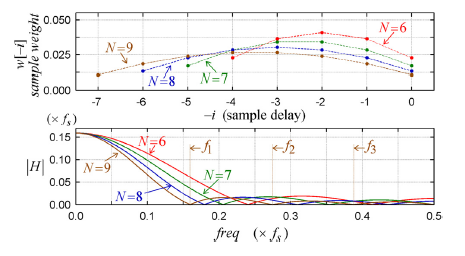
\includegraphics [scale=0.9] {f1.png}
%	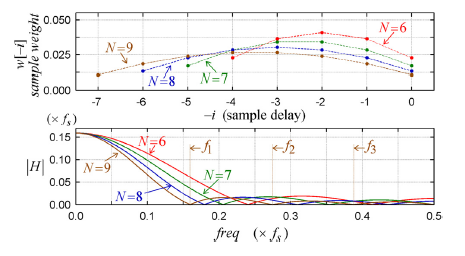
\includegraphics [width=0.9\linewidth] {f1.png}
%	\caption{Оценщик (9) веса и амплитуды частотной характеристики образца.}
%	\label{img:picture15}
%\end{figure}
%
%Три случая для вычисления $\delta$ необходимы для учета циклического характера фазового угла. Это позволяет избежать абсолютных разностей фазового угла, превышающих $\pi$ радиан.
%
%Используя \labelcref{eq:equation120}, оценка частоты сетки \labelcref{eq:equation119} выражается как:
%
%\begin{equation}\label{eq:equation121}
%\hat f_{g}[n] = \sum\limits_{i=0}^{N+2} \dfrac{3f_{s}}{4\pi} 
%\dfrac{N^2-4(i-\dfrac{1}{2}N +1)^{2}} {N(N^2 -1)} \delta[n-i] = \sum\limits_{i=0}^{N+2} f_s w [-i]\delta [n-i]
%\end{equation}
%
%где $w[-i]$ представляет вес выборки окна, примененный к каждой разности фаз и углов, задержанной на $i$ выборок$ (\delta [n - 1])$:
%
%\begin{equation}\label{eq:equation122}
%w[-i] =\dfrac{3}{4\pi} \dfrac{N^2-4(i-\dfrac{1}{2}N +1)^{2}} {N(N^2 -1)}, i=2-N, ..., -1, 0
%\end{equation}
%
%На \labelcref{img:picture15}  показан вес выборки окна \labelcref{eq:equation122} и частотная характеристика выражения \labelcref{eq:equation121} для четырех значений $ N $. Без потери общности и по соображениям ясности был выбран диапазон небольших значений $ N $. Частоты $ f_1, f_2 и f_3 $ являются частотами, для которых частотная характеристика имеет нулевое усиление для $ N = 9 $.
%
%Как уже упоминалось в \cite{kay1989fast}, \labelcref{eq:equation121} достигает Крамера-Рао для сигнала к шуму (SNR) больше, чем на 6 дБ. Это означает, что этот оценщик будет иметь лучшее подавление шума для SNR более 6 дБ. Однако этот оценщик не может полностью отклонить содержание гармоник сетки, потому что нет значения N, которое приводит к нулевому усилению на всех частотах $ f=hf_g $, где $  h $ - порядок гармоник.
%
%\subsection{Фильтрация оценки частоты с помощью фильтра скользящих средних} \label{sec:ch2/sec1_2}
%
%В общей сетке, нарушенной гармониками и дисбалансами, выражение фазового угла $ \theta $ не имеет простой замкнутой формы, как в \labelcref{eq:equation116}. Тем не менее, следующие свойства подтверждаются численным моделированием: компонент постоянного тока создает колебание фазового угла с той же частотой, что и сетка; положительная последовательность гармоники n-го порядка дает осцилляцию ошибки фазового угла $ (n - 1) $, умноженную на частоту сетки; отрицательная последовательность гармоники n-го порядка создает осцилляцию ошибки фазового угла $ (n + 1) $, умноженную на частоту сетки; значение ошибки фазового угла в течение периода сетки равно нулю. На \labelcref{img:picture16} показаны четыре примера с различными условиями сетки, где $  \theta^{1+} $- это фазовый угол основной прямой последовательности, а $ \theta $- фазовый угол, полученный из \labelcref{eq:equation116}.
%
%Фильтр скользящего среднего, применяемый к оценке частоты LMS $ ({\hat{f}}_g) $, может полностью устранить ошибки частоты из-за гармоник и дисбалансов, если длина фильтра совпадает с периодом сетки. Это происходит потому, что фильтр MAF определяется:
%
%\begin{equation}\label{eq:equation123}
%y[n] =\dfrac{1}{N} \sum\limits_{i=0}^{N-1} x [n-i]
%\end{equation}
%
%\begin{figure}[ht]
%	\centering
%	%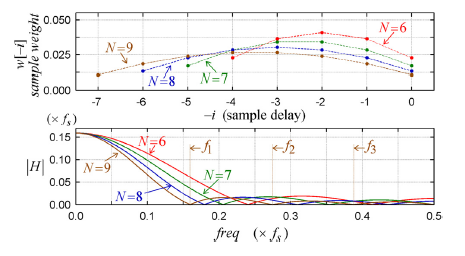
\includegraphics [scale=0.9] {f1.png}
%	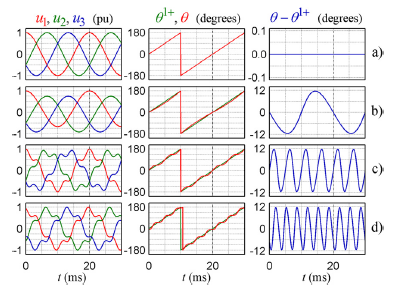
\includegraphics [width=0.9\linewidth] {f2.png}
%	\caption{Примеры фазового угла с несколькими устойчивыми состояниями сетки: (а) незагрязненный; (б) загрязнены постоянным током; (в) загрязнены положительной последовательностью 5-й гармоники и (е) загрязнены отрицательной последовательностью 5-й гармоники.}
%	\label{img:picture16}
%\end{figure}
%
%Имеет частотную характеристику с нулевой величиной в частотах, кратных обратному временному окну, то есть все сигналы в форме:
%
%\begin{equation}\label{eq:equation124}
%x[n]=a cos{(2\pi / Nkn+1)}
%\end{equation}
%
%(где $ a$ и $b $ являются действительными числами; $  N, k$ и $ n $ являются целыми числами), становятся нулевыми после фильтрации по MAF длиной N точек (y [n] = 0).
%
%Таким образом, число отсчетов MAF задается как $ N=f_s / f_g $, но это выражение действительно только тогда, когда $ f_s / f_g $ является целым числом. Поскольку в общем случае это не будет так, число выборок MAF должно быть округлено до ближайшего целого числа:
%
%\begin{equation}\label{eq:equation125}
%N=round(f_s / f_g)
%\end{equation}
%
%Однако это означает, что частотная характеристика фильтра MAF на частотах гармоник сетки больше не равна нулю, а имеет значение, которое уменьшается с увеличением $ N $, т.~е. чем больше частота дискретизации, тем меньше усиление MAF на этих частотах. На \labelcref{img:picture17} показана частотная характеристика MAF с длиной $ N = 10 $. Как и ожидалось, усиление на частоте сетки             $ f_g({0.1f}_s) $ и ее гармоники $ ({0.2f}_s,\ {0.3f}_sи {0.4f}_s) $ равны нулю. С $ N $, наложенным (13), $ |H_{MAF}| $ график действителен только для частот сетки между $ f_{g_{min}} = f_s /\ (N+0.5) $ и $ f_{g_{max}} = f_s /\ (N-0.5) $. Если $ f_g<f_{g_{min}}$ $N$ увеличивается на 1 и если $ f_g> f_{g_{max}} $ N уменьшается на 1. Таким образом, максимум $ |H_{MAF}| $ усиления происходят на частотах $ kf_{g_{min}} $ и $ {kf}_{g_{max}}$ для $ k=\left\{\ 1,\ 2,\ \ldots,\ int\left(N\ /\ 2\right)\right\} $.
%
%Следует отметить, что можно сделать $ f_s/\ f_g $ целым числом, если можно изменить частоту дискретизации. Однако предложенный оценщик частоты был разработан для управления силовыми электронными преобразователями, которые работают с фиксированной частотой PWM. Поскольку частота дискретизации связана с PWM, изменить ее невозможно.
%
%\begin{figure}[ht]
%	\centering
%	%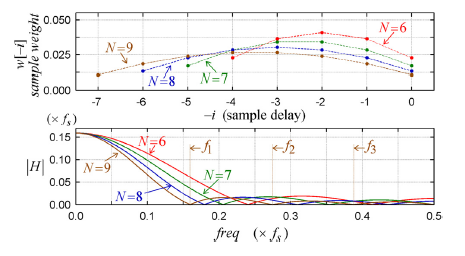
\includegraphics [scale=0.9] {f1.png}
%	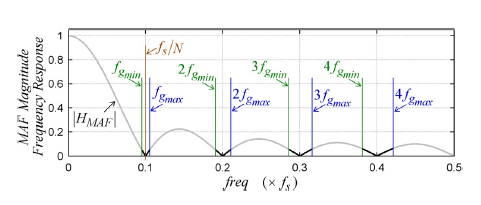
\includegraphics [width=0.9\linewidth] {f3.png}
%	\caption{Частотная характеристика фильтра скользящего среднего с длиной N=10.}
%	\label{img:picture17}
%\end{figure}
%
%\subsection{Предлагаемый метод оценки частоты сетки} \label{sec:ch2/sec1_3}
%Предлагаемое ядро оценщика состоит из фильтра MAF \labelcref{eq:equation123}, применяемого к выходу оценщика LMS \labelcref{eq:equation121}. Чтобы дать оценщику возможность работать с широкой сеткой вариаций частоты, количество выборок \labelcref{eq:equation121} и \labelcref{eq:equation123} должно быть переменным. Используя изменяющееся во времени количество выборок \labelcref{eq:equation121} и \labelcref{eq:equation123} переписываются соответственно как:
%
%\begin{equation}\label{eq:equation126}
%f\prime_g[n]= \sum\limits_{i=0}^{N_a[n]-2} \dfrac{3f_s}{4\pi} \dfrac{N_a[n]^2-4(i-\dfrac{1}{2} N_a[n]+1)^2}{N_a[n](N_a[n]^2-1)} \delta [n-i]
%\end{equation}
%
%\begin{equation}\label{eq:equation127}
%\hat{f}_g[n] =\dfrac{1}{N_b[n]}  \sum\limits_{i=0}^{N_a[n]-1} f^\prime_g[n-1]
%\end{equation}
%
%где 
%
%\begin{equation}\label{eq:equation128}
%N_a[n] = round(k_{LMS} f_s / \hat{f}_g[n-1])
%\end{equation}
%
%и
%
%\begin{equation}\label{eq:equation129}
%N_b[n] = round(k_{MAF} f_s / \hat{f}_g[n-1])
%\end{equation}
%
%представляют количество образцов, используемых \labelcref{eq:equation126} и \labelcref{eq:equation127}. $ N_a[n] $ и $ N_b[n] $ получают на основе предыдущей оценки частоты сетки $ ({\hat{f}}_g[n-1]) $, поскольку текущая оценка $ ({\hat{f}}_g[n) $ еще не доступна, когда вычисляются $ N_a[n] $ и $ N_b[n] $.
%
%Общий метод изображен на \labelcref{img:picture18}. Первым этапом является вычисление обратных разностей $ \delta $ фаз и углов сетки с использованием \labelcref{eq:equation113}, \labelcref{eq:equation116} и \labelcref{eq:equation120}. На втором этапе выполняется первая оценка частоты сетки $ (f_g^\prime) $ методом LMS с использованием \labelcref{eq:equation126}. На третьем этапе получают оценку частоты сетки $ ({\hat{f}}_g) $ путем фильтрации первой оценки с использованием фильтра MAF с использованием \labelcref{eq:equation127}. Количество выборок в \labelcref{eq:equation126} и \labelcref{eq:equation127} определяется расчетной частотой сетки.
%
%Следует отметить, что дифференциатор LMS \labelcref{eq:equation119}, применяемый к фазовому углу, реализуется с помощью \labelcref{eq:equation120} и \labelcref{eq:equation126}.
%
%Оценщик в виде двух параметров: $ k_{LMS} $ и $ k_{MAF} $. Параметр $ k_{MAF} $ установлен в 1, так как это минимальное значение, которое позволяет отклонять гармонические помехи. Устанавливая это значение на минимум, время установления также сохраняется на минимуме. Однако для улучшения подавления гармоник, особенно если $ f_s/\ f_g $ не является целым числом, $ k_{MAF} $ может быть установлено на большее целое число. Недостатком является снижение динамики, увеличивающее время установления оценки.
%
%Параметр $ k_{LMS} $ устанавливается для минимизации влияния гармоник напряжения сети и дисбалансов в оценке частоты, как описано в следующем подразделе.
%
%\subsection{Метод выбора алгоритма LMS по количеству выборок} \label{sec:ch2/sec1_4}
%
%Чтобы выбрать значение параметра $ k_{LMS} $, анализируются коэффициенты усиления частотного отклика в частотах гармоник. Выбранный критерий состоит в том, чтобы минимизировать квадратный корень из суммы квадратов усиления $ (J_H) $ на этих частотах:
%
%\begin{figure}[ht]
%	\centering
%	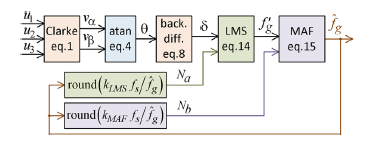
\includegraphics [width=0.9\linewidth] {f4.png}
%	\caption{Схема предлагаемого способа оценки частоты сетки.}
%	\label{img:picture18}
%\end{figure}
%
%\begin{equation}\label{eq:equation130}
%J_H=\sqrt{\sum_{h=1}^{h_{max}}{H^2(hf_g),}}\ \ \ \ \ \ \ h_{max}=int(\frac{1}{2}f_s/\ f_g)
%\end{equation}
%
%где функция int (x) возвращает целую часть числа x. Гармоника $ h_{max} $- это максимальный порядок гармоник основной частоты $ f_g $, который можно анализировать с частотой дискретизации $ f_s $.
%
%В качестве примера на \labelcref{img:picture19} показаны частотные характеристики оценщика LMS $ (H_{LMS}) $, фильтра MAF $ (H_{MAF}) $ и полного оценщика $ (H) $ для заданного набора значений $ f_s $, $ N_a $ и $ N_b $. Точки представляют коэффициенты усиления в гармониках для данной частоты сетки: $ f_g=52.6 Гц $. Сумма квадратов усиления должна быть минимизирована путем правильного выбора $ N_a $.
%
%На \labelcref{img:picture20} показана эволюция $ J_H $ как функции параметра $ N_a $ для тех же значений $ f_s $, $ N_b $ и $ f_g $, что и на \labelcref{img:picture19}. Функция имеет два локальных минимума (для показанного диапазона $ N_a $): $ N_a=14 $ и $ N_a=24 $. Чтобы улучшить динамику оценки (сократить время установления), выбирается нижнее значение: $ N_a=14 $. Следует отметить, что если частота дискретизации кратна частоте сетки, точки, представленные на \labelcref{img:picture19} будет соответствовать нулям MAF, а значение $ J_H $ на \labelcref{img:picture20} всегда будет равно нулю.
%
%Чтобы получить выражение для значения  $ N_a $ как функции от $ f_s $ и $ f_g $, было выполнено несколько симуляций, как показано на \labelcref{img:picture20}. Моделирование для частоты сетки между 30 Гц и 70 Гц (с шагом 1 МГц) и для частоты дискретизации между 500 Гц и 10 кГц (с шагом 50 Гц) позволяет сделать вывод, что значение $ N_a $, которое минимизирует $  J_H $, составляет:
%
%\begin{equation}\label{eq:equation131}
%N_a=round(1.431 f_s / f_g)
%\end{equation}
%
%и так, параметр $ k_{LMS} $ установлен в:
%
%\begin{equation}\label{eq:equation132}
%k_{LMS}=1.431
%\end{equation}
%
%\labelcref{img:picture21} иллюстрирует эволюцию величины $ J_H $ и число выборок, используемых устройство оценки LMS $ (N_a) $, и с помощью фильтра MAF $ (N_b) $ в зависимости от частоты сетки для конкретной частоты дискретизации с использованием 
%$ k_{LMS}=1.431 $ и $ k_{MAF}=1 $.
%
%\begin{figure}[ht]
%	\centering
%	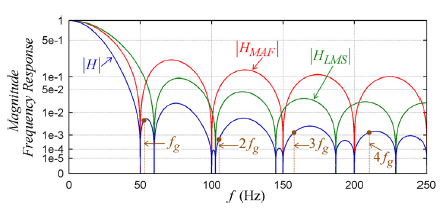
\includegraphics [width=0.9\linewidth] {f5.png}
%	\caption{Частотные характеристики оценки LMS $ (H_{LMS}) $, фильтра MAF $ (H_{MAF}) $ и полной оценки (H) для $ f_s=500 Гц $, $ N_a=12 $ и $ N_b=10 $. $ (vertical\ scale\ =\ x^{1/5}) $.}
%	\label{img:picture19}
%\end{figure}
%
%\begin{figure}[ht]
%	\centering
%	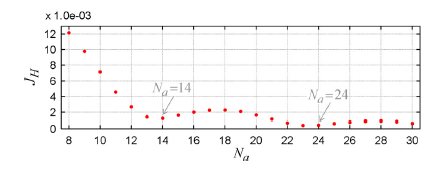
\includegraphics [width=0.9\linewidth] {f6.png}
%	\caption{Эволюция $ J_H $ как функция параметра $ N_a $ для $ f_s=500 Гц $, 
%		$ N_b=10 $ и $ f_s=52.6 Гц $.}
%	\label{img:picture20}
%\end{figure}
%
%\begin{figure}[ht]
%	\centering
%	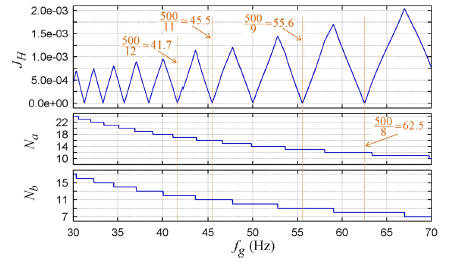
\includegraphics [width=0.9\linewidth] {f7.png}
%	\caption{Эволюция $ J_H $, $  N_a $ и $ N_b $ как функция частоты сетки для $ f_s=500 Гц $.}
%	\label{img:picture21}
%\end{figure}
%
%Значение $ J_H $ равно нулю всякий раз, когда $ f_g $ является фактором $ f_s $. Локальные максимумы $ J_H $ увеличиваются с увеличением частоты сетки.
%
%\subsection{Рекурсивная реализация} \label{sec:ch2/sec1_5}
%
%Чтобы улучшить вычислительные требования оценщика за счет сокращения количества операций и времени выполнения, должна использоваться рекурсивная реализация.
%
%Оценщик частоты LMS в \labelcref{eq:equation126} может быть выражен как:
%
%\begin{equation}\label{eq:equation133}
%f_g^\prime[n]=\frac{3f_s}{\pi} \dfrac{(N_a[n]-1) S_\delta[n] +(N_a[n]-2) S_{i \delta}[n] - S_{i^2 \delta[n]}} {N_a[n] (N_a[n]^2-1}
%\end{equation}
%
%где 
%
%\begin{equation}\label{eq:equation134}
%S_\delta[n] = \sum_{i=0}^{N_a[n]-2} \delta[n-i]
%\end{equation}
%
%\begin{equation}\label{eq:equation135}
%S_{i\delta}[n] = \sum_{i=0}^{N_a[n]-2} \delta[n-i]
%\end{equation}
%
%и 
%
%\begin{equation}\label{eq:equation136}
%S_{i^2\delta}[n] = \sum_{i=0}^{N_a[n]-2} i^2\delta[n-i]
%\end{equation}
%
%Фильтр MAF в \labelcref{eq:equation127} можно переписать как:
%
%\begin{equation}\label{eq:equation137}
%\hat{f}_g[n] = S_{\hat{f}_g} [n] / N_b[n]
%\end{equation}
%
%где 
%
%\begin{equation}\label{eq:equation138}
%S_{\hat{f}_g} [n] = \sum_{i=0}^{N_a[n]-1} \hat{f}_g [n-i]
%\end{equation}
%
%Если различия $ N_a $ и $ N_b $  между последовательными циклами ограничены до $ ±1 $, суммы $ S_{f_g^\prime}[n] $ могут быть реализованы рекурсивно. Несколько симуляций показали, что различия находятся в этом диапазоне даже при наличии частотного шага для частот дискретизации выше 500 Гц. Однако, если это условие не выполняется, рекурсивный алгоритм все еще работает должным образом, ограничивая различия до $ ±1 $ замедляя обновление $ N_a $ и  $ N_b $.
%
%Принимая во внимание это соображение, необходимы три случая, чтобы учесть изменения $ N_a $ и $ N_b $ в суммах, определенных рекурсивно. Рекурсивные версии \labelcref{eq:equation134} - \labelcref{eq:equation137} определяются соответственно \labelcref{eq:equation139} -  \labelcref{eq:equation142}:
%
%\begin{equation}\label{eq:equation139}
%\footnotesize{
%S_\delta[n]=
%\begin{cases}
%S_\delta[n-1]+\delta[n]-\delta_{n1}-\delta_{n2} , &\text{если $N_a[n]=N_a[n-1]-1$} \\
%S_\delta[n-1]+\delta[n]-\delta_{n1} , &\text{если $N_a[n]=N_a[n-1]$} \\
%S_\delta[n-1]+\delta[n] , &\text{если $N_a[n]=N_a[n-1]+1$}
%\end{cases}
%}
%\end{equation}
%
%\begin{equation}\label{eq:equation140}
%\footnotesize{
%S_{i\delta}[n]=
%\begin{cases}
%S_{i\delta}[n-1]+S_\delta[n-1]-k_1 \delta_{n1}-k_2 \delta_{n2} , &\text{если $N_a[n]=N_a[n-1]-1$} \\
%S_{i\delta}[n-1]+S_\delta[n-1]-k_1 \delta_{n1}, &\text{если $N_a[n]=N_a[n-1]$} \\
%S_{i\delta}[n-1]+S_\delta[n-1] , &\text{если $N_a[n]=N_a[n-1]+1$}
%\end{cases}
%}
%\end{equation}
%
%\begin{equation}\label{eq:equation141}
%\footnotesize{
%S_{i^{2}\delta}[n]=
%\begin{cases}
%S_{i^2\delta}[n-1]+{2S}_{i\delta}[n-1]+S_\delta[n-1]-k_1^2\delta_{n1}-k_2^2\delta_{n2} , &\text{если $N_a[n]=N_a[n-1]-1$} \\
%S_{i^2\delta}[n-1]+{2S}_{i\delta}[n-1]+S_\delta[n-1]-k_1^2\delta_{n1}, &\text{если $N_a[n]=N_a[n-1]$} \\
%S_{i^2\delta}[n-1]+{2S}_{i\delta}[n-1]+S_\delta[n-1] , &\text{если $N_a[n]=N_a[n-1]+1$}
%\end{cases}
%}
%\end{equation}
%
%И 
%
%\begin{equation}\label{eq:equation142}
%\footnotesize{
%S_{f^\prime_g}[n]=
%\begin{cases}
%S_{f^\prime_g}[n-1] + f^\prime_g[n] + f^\prime_g[n-N_b[n]] - f^\prime_g[n-N_b[n]-1] , &\text{если $N_a[n]=N_a[n-1]-1$} \\
%S_{f^\prime_g}[n-1] + f^\prime_g[n] + f^\prime_g[n-N_b[n]], &\text{если $N_a[n]=N_a[n-1]$} \\
%S_{f^\prime_g}[n-1] + f^\prime_g[n] , &\text{если $N_a[n]=N_a[n-1]+1$}
%\end{cases}
%}
%\end{equation}
%
%где $ k_1=1-N_a[n] $, $ k_2=N_a[n] $, $ \delta_{n1}=\delta[n-N_a[n]+1] $ и $ \delta_{n2}=\delta[n-N_a[n]] $
%
%Реализация алгоритма с использованием рекурсивных и циклических буферов показана в Алгоритме 1. Алгоритм написан с использованием записи Octave / Matlab и является готовой к использованию функцией. Однако алгоритм не использует какие-либо конкретные функции Octave / Matlab, которые легко адаптируются к другим языкам программирования. При использовании метода циклического буфера оптимизируется время выполнения для доступа к значениям переменных в предыдущих циклах. Если линейно-нейтральные напряжения недоступны, алгоритм может использоваться с линейно-линейными напряжениями путем правильной настройки строки алгоритма с номером 20.
%
%\begin{figure}[ht]
%	\centering
%	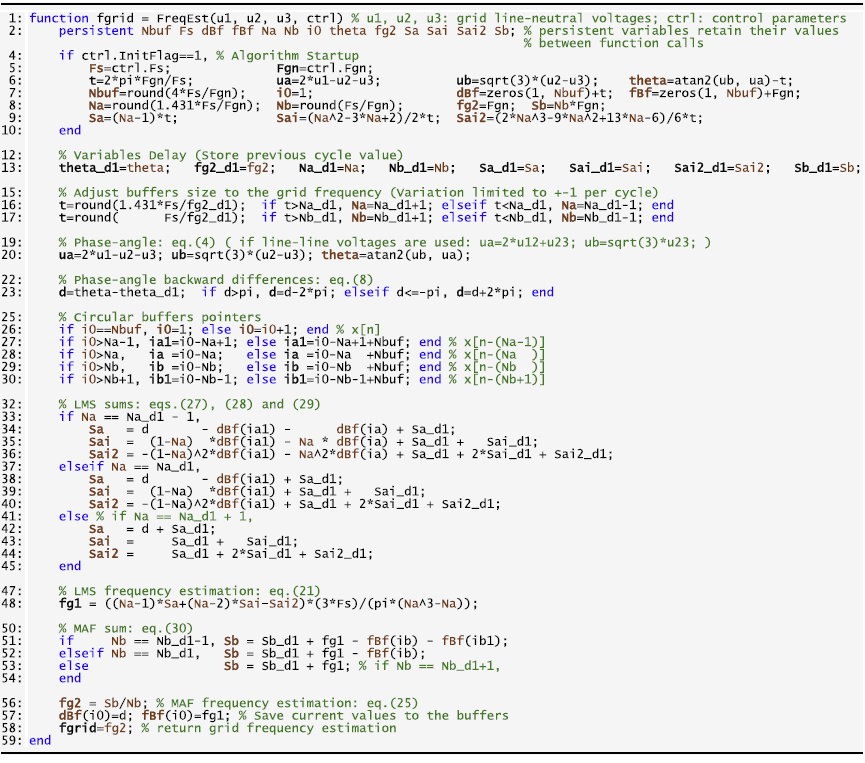
\includegraphics [width=0.9\linewidth] {a1.png}
%	\caption{Алгоритм 1.}
%	\label{img:picture22}
%\end{figure}
%
%\begin{table} [htbp]
%	\centering
%	\caption{Параметры оценщиков.}%
%	\label{tab:makecell}%
%	\begin{tabular}{| c  c  c  c  c |}
%		\hline
%		% 1 строка
%		%Колонка 1.1 
%		LMSD & 
%		%Колонка 1.2
%		WLLMP &
%		%Колонка 1.3
%		IRNTA & 
%		%Колонка 1.4
%		FLMS &
%		%Колонка 1.5
%		DMD \\ \hline
%
%		% 2 строка
%		\multicolumn{1}{|c}{\thead{$k_{LMS}  = 1.431$}} & \multicolumn{1}{c}{\thead{Размер шага:}} & \multicolumn{1}{c}{\thead{Фактор забвения}} & \multicolumn{1}{c}{\thead{$\mu_{max} =0.024$}} & \multicolumn{1}{c|}{\thead{DFT:}} \\ \hline
%		
%        % 3 строка
%	    \multicolumn{1}{|c}{\thead{$k_{MAF} = 1$}} & \multicolumn{1}{c}{\thead{$ \mu=0.048$}} & \multicolumn{1}{c}{\thead{$\lambda =0.9645$}} & \multicolumn{1}{c}{\thead{$\mu_{min} =0.001$}} & \multicolumn{1}{c|}{\thead{$h_1:$ один \\ цикл треугольный}} \\ \hline
%	    
%	    % 4 строка
%	    \multicolumn{2}{|c}{} & \multicolumn{1}{c}{\thead{Начальное значение \\ ковариации}} & \multicolumn{1}{c}{\thead{$\lambda =0.97$}} & \multicolumn{1}{c|}{\thead{\thead{Сглаживающий \\ фильтр:}}}  \\ \hline
%	   
%		% 5 строка
%		\multicolumn{2}{|c}{} & \multicolumn{1}{c}{\thead{$\delta = 100$}} & \multicolumn{1}{c}{\thead{$\gamma =0.01$}} & \multicolumn{1}{c|}{\thead{\thead{$h_1:$ один  двухтактный \\ фильтр Кея}}}  \\ \hline
%			   
%	   
%	    % 6 строка
%		\multicolumn{3}{|c}{} & \multicolumn{1}{c}{\thead{$\rho=0.99$}} & \multicolumn{1}{c|}{}  \\ \hline
%	\end{tabular}%
%\end{table}

